\documentclass[runningheads]{llncs}
\usepackage{graphicx}
\usepackage[text={150mm,220mm},centering,nohead]{geometry}
\usepackage{listings}

\usepackage{color}
\definecolor{gray}{rgb}{0.4,0.4,0.4}
\definecolor{darkblue}{rgb}{0.0,0.0,0.6}
\definecolor{cyan}{rgb}{0.0,0.6,0.6}

\lstset{
  basicstyle=\ttfamily,
  columns=fullflexible,
  showstringspaces=false,
  commentstyle=\color{gray}\upshape
}
\lstset{breaklines}
\lstdefinelanguage{XML}
{
  morestring=[b]",
  morestring=[s]{>}{<},
  morecomment=[s]{<?}{?>},
  stringstyle=\color{black},
  identifierstyle=\color{darkblue},
  keywordstyle=\color{cyan},
  morekeywords={xmlns,version,type}% list your attributes here
}
\pagestyle{empty}
\begin{document}
\title{\large{CSCI927 Service-Oriented Software Engineering (Progress Report)}}
\author{}
\institute{}
\maketitle
\vspace{-1cm}
%-----------Please Do NOT change the content above.-----------------

%---------------------------------------------------------------------------------------------------------------------------------

%-----------Please write the project information here.---------------

\begin{center}
\Large{\textbf{Online study lounge system based on SOA}} \\ % Please write your project tile in here
\vspace{0.2cm}
\large{\emph{ Liting Lyu (6603324), Yueyue  He (6603671), Muzhe Peng (6603646), Wangzhihui Mei (6603385)}}\\%Please write names of your group members as well as the group number in here
\vspace{0.3cm}
\end{center}

%-----------Please write the content of your research proposal from here.---------------
\noindent %peng muzhe
\section*{Progress}
\subsection*{}
In order to better description the service, the model is further designed according to the proposal. The must-have modules have finished designing, which includes Updates Issue module, Search module and Message Processing Module. The technology of Business Process Modeling Notation(BPMN) and corresponding Extensive Markup Language(XML) are used to denote well-organized and predictable process, Case Management Model and Notation(CMMN) is used to describe the unpredictable process. More details are included in the appendix. 
\\Slight adjustment is made to make the function of the service more appropriate, which is:
\\Deleting the Updates Searching module in the Search service. Because the online study lounge system should focus more on helping users form good habits for study, however it seems unnecessary to search for a certain updates, this module will divert users’ attention more on friends making. 


\subsection*{Q\&A Module} %maywzh
\noindent
For Q\&A module, We have developed Question Service and Answer Service along with interaction with Follow Service, Push Service. Down-top design was used to build the system, dividing the application into two layer: basic layer and business logic layer. The SOA pattern was referred in building the System, dividing Question Services and Answer Services into atomic services. BPMN model was used to describe the business process model of the Q\&A module in the view of users. Also, We use CMMN model to describe the case model of the moduel. The according xml files are offered.
Generating Question Services consists search question service, add/edit/follow question services and follow question service, we considered the general business model of the service and combined them into a whold model. In CMMN Model, We connected Question Service and Answer Service, to show the whole service chain.

\section*{Next plan}
1.Design the good-to-have services
\\2.Try to apply more technology.

\clearpage
\begin{flushleft}
    \huge{\textbf{Appendix}}
\end{flushleft}
\begin{center}
    \Large{\textbf{Project Title: Online study lounge system based on SOA }} \\*[0.1cm]%Please write names of the project title in here
    \large{\emph{Group Members (Group number): Liting Lyu (6603324), Yueyue  He (6603671), Muzhe Peng (6603646), Wangzhihui Mei (6603385)}} %Please write names of your group members as well as the group number in here
\end{center}
    %----------------------------------------------------------------------------------------------------------------------------
    
    %-----------Please write the content of your appendix (diagrams, figures, tables, etc) from here.---------------
    %maywzh

	\textbf{Question Service BPMN Model and XML}\\
	\begin{figure}
		\centering %图片居中
		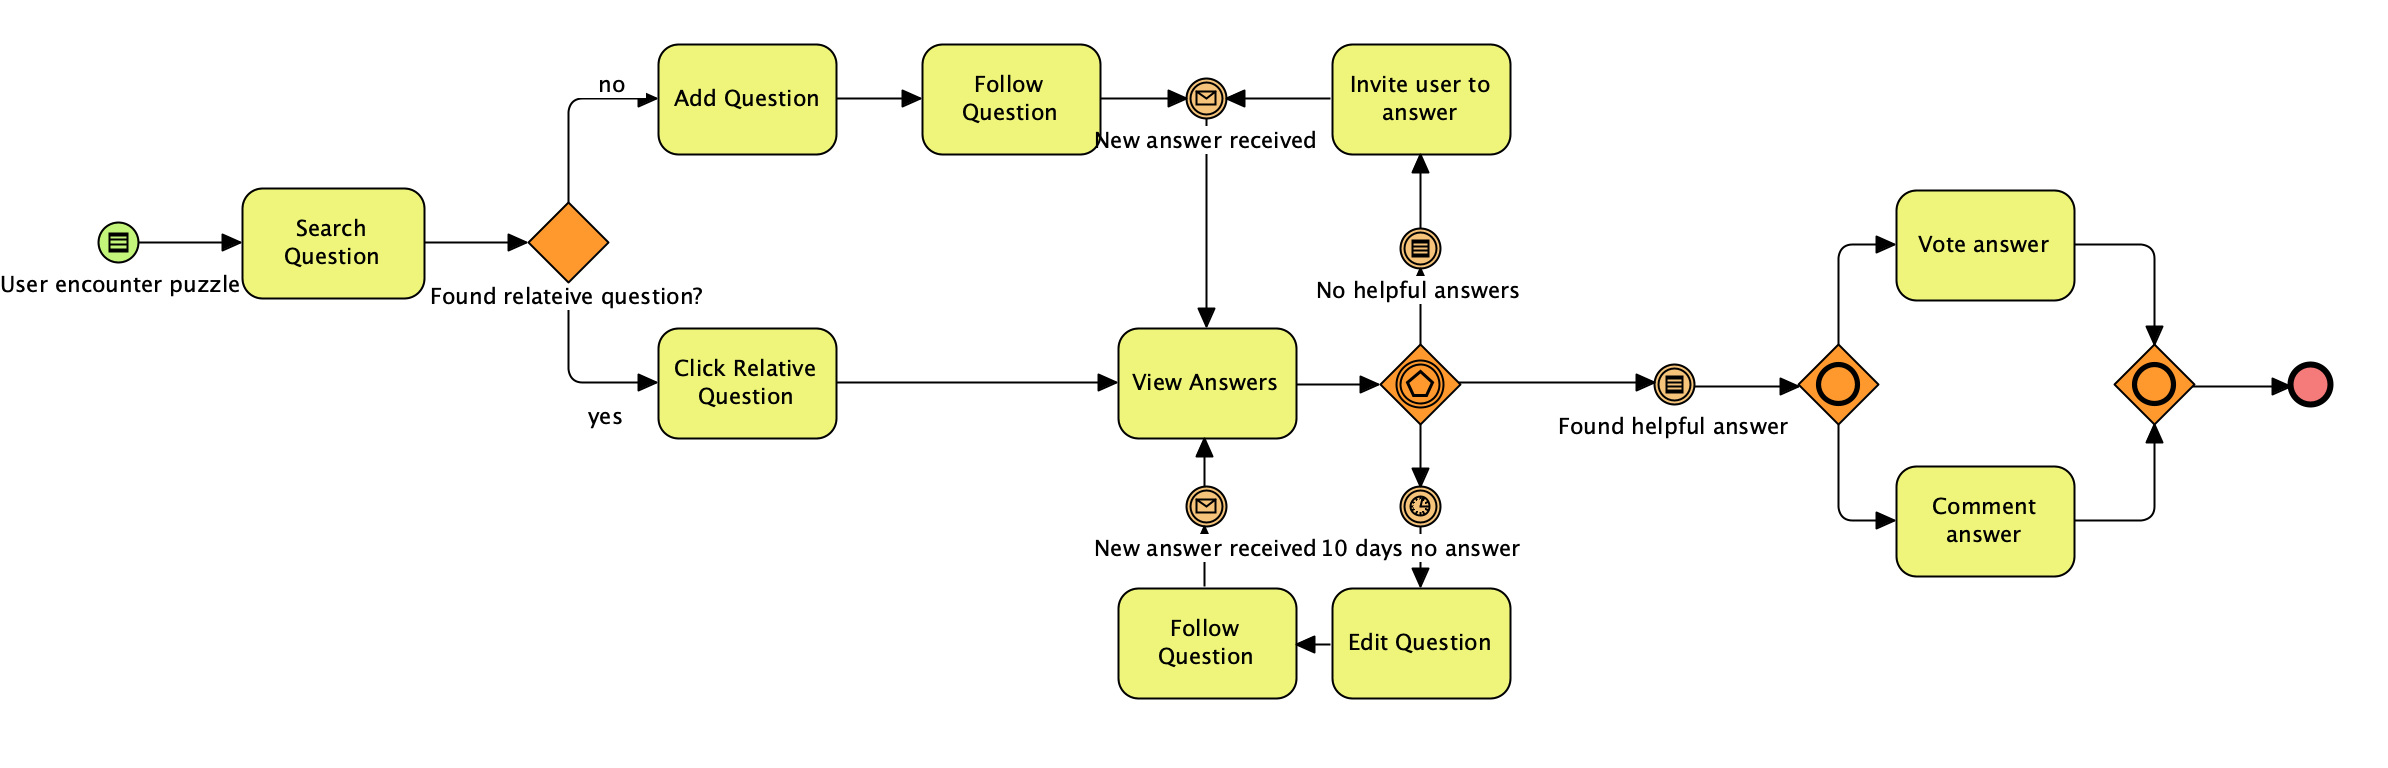
\includegraphics[width=1.0\textwidth]{figure/mwzh/questionservice} %插入图片,[]中设置图片大小,{}中是图片文件名
		\caption{Question Service} %最终文档中希望显示的图片标题
		\label{questionservice} %用于文内引用的标签
	\end{figure}
    \noindent 
    \begin{lstlisting}[language={XML}]
        <process id="_1" isExecutable="false" name="QuestionService">
		<task completionQuantity="1" id="BP06_BP12" isForCompensation="false" name="Search Question">
			<incoming>BP06_BP22</incoming>
			<outgoing>BP06_BP24</outgoing>
		</task>
		<startEvent id="BP06_BP13" isInterrupting="true" name="User encounter puzzle">
			<outgoing>BP06_BP22</outgoing>
			<conditionalEventDefinition id="ID_14404272_1627_3203_7600_000000200040">
				<condition/>
			</conditionalEventDefinition>
		</startEvent>
		<sequenceFlow id="BP06_BP22" name="" sourceRef="BP06_BP13" targetRef="BP06_BP12"/>
		<exclusiveGateway gatewayDirection="Unspecified" id="BP06_BP23" name="Found relateive question?">
			<incoming>BP06_BP24</incoming>
			<outgoing>BP06_BP29</outgoing>
			<outgoing>BP06_BP30</outgoing>
		</exclusiveGateway>
		<sequenceFlow id="BP06_BP24" name="" sourceRef="BP06_BP12" targetRef="BP06_BP23"/>
		<task completionQuantity="1" id="BP06_BP27" isForCompensation="false" name="Add Question">
			<incoming>BP06_BP29</incoming>
			<outgoing>BP06_BP40</outgoing>
		</task>
		<task completionQuantity="1" id="BP06_BP28" isForCompensation="false" name="Click Relative Question">
			<incoming>BP06_BP30</incoming>
			<outgoing>BP06_BP43</outgoing>
		</task>
		<sequenceFlow id="BP06_BP29" name="no" sourceRef="BP06_BP23" targetRef="BP06_BP27"/>
		<sequenceFlow id="BP06_BP30" name="yes" sourceRef="BP06_BP23" targetRef="BP06_BP28"/>
		<task completionQuantity="1" id="BP06_BP37" isForCompensation="false" name="View Answers">
			<incoming>BP06_BP43</incoming>
			<incoming>BP06_BP44</incoming>
			<incoming>BP06_BP88</incoming>
			<outgoing>BP06_BP71</outgoing>
		</task>
		<task completionQuantity="1" id="BP06_BP39" isForCompensation="false" name="Follow Question">
			<incoming>BP06_BP40</incoming>
			<outgoing>BP06_BP42</outgoing>
		</task>
		<sequenceFlow id="BP06_BP40" name="" sourceRef="BP06_BP27" targetRef="BP06_BP39"/>
		<intermediateCatchEvent id="BP06_BP41" name="New answer received">
			<incoming>BP06_BP42</incoming>
			<incoming>BP06_BP62</incoming>
			<outgoing>BP06_BP44</outgoing>
			<messageEventDefinition id="ID_54404272_1627_3203_7600_000000200041"/>
		</intermediateCatchEvent>
		<sequenceFlow id="BP06_BP42" name="" sourceRef="BP06_BP39" targetRef="BP06_BP41"/>
		<sequenceFlow id="BP06_BP43" name="" sourceRef="BP06_BP28" targetRef="BP06_BP37"/>
		<sequenceFlow id="BP06_BP44" name="" sourceRef="BP06_BP41" targetRef="BP06_BP37"/>
		<endEvent id="BP06_BP45" name="">
			<incoming>BP06_BP69</incoming>
		</endEvent>
		<inclusiveGateway gatewayDirection="Unspecified" id="BP06_BP51" name="Gateway">
			<incoming>BP06_BP73</incoming>
			<outgoing>BP06_BP55</outgoing>
			<outgoing>BP06_BP65</outgoing>
		</inclusiveGateway>
		<task completionQuantity="1" id="BP06_BP53" isForCompensation="false" name="Comment answer">
			<incoming>BP06_BP55</incoming>
			<outgoing>BP06_BP68</outgoing>
		</task>
		<sequenceFlow id="BP06_BP55" name="" sourceRef="BP06_BP51" targetRef="BP06_BP53"/>
		<task completionQuantity="1" id="BP06_BP60" isForCompensation="false" name="Invite user to answer">
			<incoming>BP06_BP77</incoming>
			<outgoing>BP06_BP62</outgoing>
		</task>
		<sequenceFlow id="BP06_BP62" name="" sourceRef="BP06_BP60" targetRef="BP06_BP41"/>
		<task completionQuantity="1" id="BP06_BP64" isForCompensation="false" name="Vote answer">
			<incoming>BP06_BP65</incoming>
			<outgoing>BP06_BP67</outgoing>
		</task>
		<sequenceFlow id="BP06_BP65" name="" sourceRef="BP06_BP51" targetRef="BP06_BP64"/>
		<inclusiveGateway gatewayDirection="Unspecified" id="BP06_BP66" name="Gateway2">
			<incoming>BP06_BP67</incoming>
			<incoming>BP06_BP68</incoming>
			<outgoing>BP06_BP69</outgoing>
		</inclusiveGateway>
		<sequenceFlow id="BP06_BP67" name="" sourceRef="BP06_BP64" targetRef="BP06_BP66"/>
		<sequenceFlow id="BP06_BP68" name="" sourceRef="BP06_BP53" targetRef="BP06_BP66"/>
		<sequenceFlow id="BP06_BP69" name="" sourceRef="BP06_BP66" targetRef="BP06_BP45"/>
		<eventBasedGateway gatewayDirection="Unspecified" id="BP06_BP70" instantiate="false" name="">
			<incoming>BP06_BP71</incoming>
			<outgoing>BP06_BP76</outgoing>
			<outgoing>BP06_BP78</outgoing>
			<outgoing>BP06_BP80</outgoing>
		</eventBasedGateway>
		<sequenceFlow id="BP06_BP71" name="" sourceRef="BP06_BP37" targetRef="BP06_BP70"/>
		<intermediateCatchEvent id="BP06_BP72" name="Found helpful answer">
			<incoming>BP06_BP78</incoming>
			<outgoing>BP06_BP73</outgoing>
			<conditionalEventDefinition id="ID_01527216_1627_3203_7600_000000200061">
				<condition/>
			</conditionalEventDefinition>
		</intermediateCatchEvent>
		<sequenceFlow id="BP06_BP73" name="" sourceRef="BP06_BP72" targetRef="BP06_BP51"/>
		<intermediateCatchEvent id="BP06_BP74" name="No helpful answers">
			<incoming>BP06_BP76</incoming>
			<outgoing>BP06_BP77</outgoing>
			<conditionalEventDefinition id="ID_01527216_1627_3203_7600_000000200062">
				<condition/>
			</conditionalEventDefinition>
		</intermediateCatchEvent>
		<intermediateCatchEvent id="BP06_BP75" name="10 days no answer">
			<incoming>BP06_BP80</incoming>
			<outgoing>BP06_BP82</outgoing>
			<timerEventDefinition id="ID_01527216_1627_3203_7600_000000200063"/>
		</intermediateCatchEvent>
		<sequenceFlow id="BP06_BP76" name="" sourceRef="BP06_BP70" targetRef="BP06_BP74"/>
		<sequenceFlow id="BP06_BP77" name="" sourceRef="BP06_BP74" targetRef="BP06_BP60"/>
		<sequenceFlow id="BP06_BP78" name="" sourceRef="BP06_BP70" targetRef="BP06_BP72"/>
		<sequenceFlow id="BP06_BP80" name="" sourceRef="BP06_BP70" targetRef="BP06_BP75"/>
		<task completionQuantity="1" id="BP06_BP81" isForCompensation="false" name="Edit Question">
			<incoming>BP06_BP82</incoming>
			<outgoing>BP06_BP84</outgoing>
		</task>
		<sequenceFlow id="BP06_BP82" name="" sourceRef="BP06_BP75" targetRef="BP06_BP81"/>
		<task completionQuantity="1" id="BP06_BP83" isForCompensation="false" name="Follow Question">
			<incoming>BP06_BP84</incoming>
			<outgoing>BP06_BP87</outgoing>
		</task>
		<sequenceFlow id="BP06_BP84" name="" sourceRef="BP06_BP81" targetRef="BP06_BP83"/>
		<intermediateCatchEvent id="BP06_BP86" name="New answer received">
			<incoming>BP06_BP87</incoming>
			<outgoing>BP06_BP88</outgoing>
			<messageEventDefinition id="ID_41527216_1627_3203_7600_000000200064"/>
		</intermediateCatchEvent>
		<sequenceFlow id="BP06_BP87" name="" sourceRef="BP06_BP83" targetRef="BP06_BP86"/>
		<sequenceFlow id="BP06_BP88" name="" sourceRef="BP06_BP86" targetRef="BP06_BP37"/>
	</process>
    
	\end{lstlisting}
	\clearpage
	\textbf{Answer Service BPMN Model and XML}\\
	\begin{figure}
		\centering %图片居中
		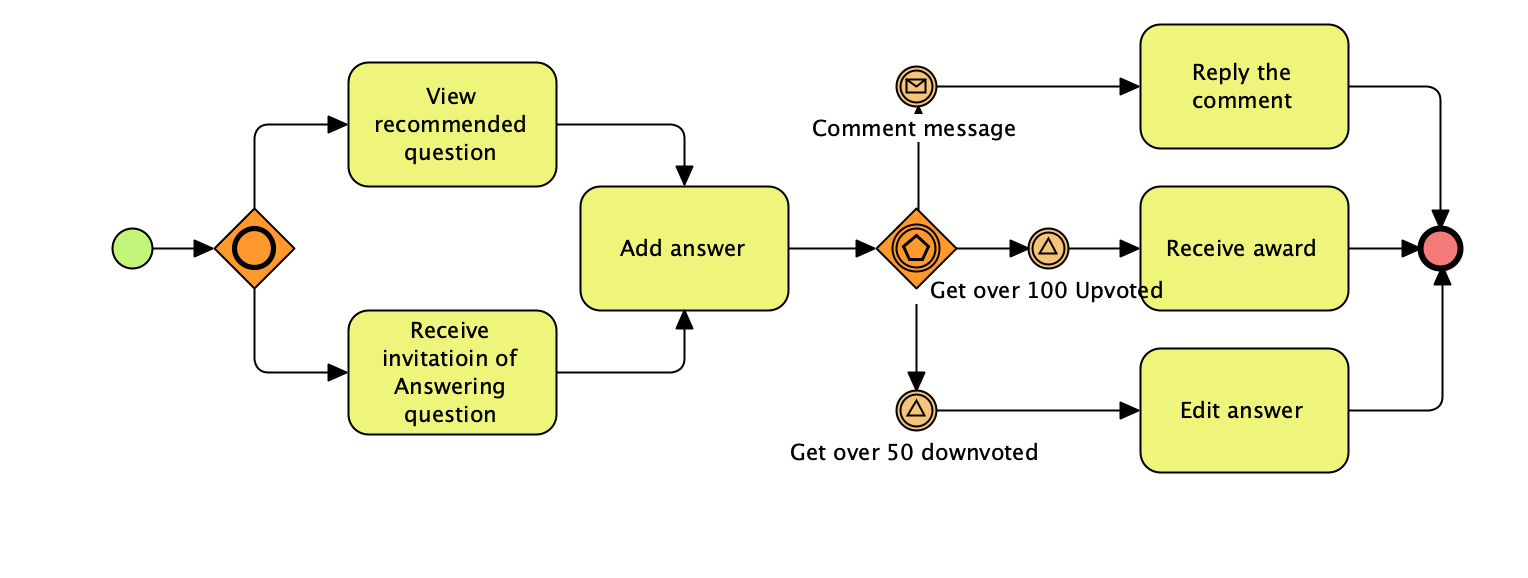
\includegraphics[width=1.0\textwidth]{figure/mwzh/answerservice} %插入图片,[]中设置图片大小,{}中是图片文件名
		\caption{Answer Service} %最终文档中希望显示的图片标题
		\label{answerservice} %用于文内引用的标签
	\end{figure}
	\begin{lstlisting}[language={XML}]
		<process id="_4" isExecutable="false" name="AnswerService">
		<task completionQuantity="1" id="BP80_BP02" isForCompensation="false" name="View recommended question" startQuantity="1">
			<incoming>BP80_BP27</incoming>
			<outgoing>BP80_BP05</outgoing>
		</task>
		<task completionQuantity="1" id="BP80_BP04" isForCompensation="false" name="Add answer" startQuantity="1">
			<incoming>BP80_BP05</incoming>
			<incoming>BP80_BP29</incoming>
			<outgoing>BP80_BP11</outgoing>
		</task>
		<sequenceFlow id="BP80_BP05" name="" sourceRef="BP80_BP02" targetRef="BP80_BP04" />
		<eventBasedGateway gatewayDirection="Unspecified" id="BP80_BP10" instantiate="false" name="">
			<incoming>BP80_BP11</incoming>
			<outgoing>BP80_BP17</outgoing>
			<outgoing>BP80_BP16</outgoing>
			<outgoing>BP80_BP34</outgoing>
		</eventBasedGateway>
		<sequenceFlow id="BP80_BP11" name="" sourceRef="BP80_BP04" targetRef="BP80_BP10" />
		<task completionQuantity="1" id="BP80_BP12" isForCompensation="false" name="Reply the comment" startQuantity="1">
			<incoming>BP80_BP19</incoming>
			<outgoing>BP80_BP40</outgoing>
		</task>
		<intermediateCatchEvent id="BP80_BP13" name="Comment message">
			<incoming>BP80_BP17</incoming>
			<outgoing>BP80_BP19</outgoing>
			<messageEventDefinition id="ID_47301753_1627_3203_7600_000000200121" />
		</intermediateCatchEvent>
		<sequenceFlow id="BP80_BP17" name="" sourceRef="BP80_BP10" targetRef="BP80_BP13" />
		<sequenceFlow id="BP80_BP19" name="" sourceRef="BP80_BP13" targetRef="BP80_BP12" />
		<task completionQuantity="1" id="BP80_BP23" isForCompensation="false" name="Receive invitatioin of Answering question" startQuantity="1">
			<incoming>BP80_BP28</incoming>
			<outgoing>BP80_BP29</outgoing>
		</task>
		<startEvent id="BP80_BP24" name="">
			<outgoing>BP80_BP26</outgoing>
		</startEvent>
		<inclusiveGateway gatewayDirection="Unspecified" id="BP80_BP25" name="">
			<incoming>BP80_BP26</incoming>
			<outgoing>BP80_BP27</outgoing>
			<outgoing>BP80_BP28</outgoing>
		</inclusiveGateway>
		<sequenceFlow id="BP80_BP26" name="" sourceRef="BP80_BP24" targetRef="BP80_BP25" />
		<sequenceFlow id="BP80_BP27" name="" sourceRef="BP80_BP25" targetRef="BP80_BP02" />
		<sequenceFlow id="BP80_BP28" name="" sourceRef="BP80_BP25" targetRef="BP80_BP23" />
		<sequenceFlow id="BP80_BP29" name="" sourceRef="BP80_BP23" targetRef="BP80_BP04" />
		<sequenceFlow id="BP80_BP16" name="" sourceRef="BP80_BP10" targetRef="BP80_BP14" />
		<intermediateCatchEvent id="BP80_BP14" name="Get over 100 Upvoted">
			<incoming>BP80_BP16</incoming>
			<outgoing>BP80_BP32</outgoing>
			<signalEventDefinition id="ID_27301753_1627_3203_7600_000000200122" />
		</intermediateCatchEvent>
		<task completionQuantity="1" id="BP80_BP31" isForCompensation="false" name="Receive award" startQuantity="1">
			<incoming>BP80_BP32</incoming>
			<outgoing>BP80_BP41</outgoing>
		</task>
		<sequenceFlow id="BP80_BP32" name="" sourceRef="BP80_BP14" targetRef="BP80_BP31" />
		<intermediateCatchEvent id="BP80_BP33" name="Get over 50 downvoted">
			<incoming>BP80_BP34</incoming>
			<outgoing>BP80_BP36</outgoing>
			<signalEventDefinition id="ID_27301753_1627_3203_7600_000000200123" />
		</intermediateCatchEvent>
		<sequenceFlow id="BP80_BP34" name="" sourceRef="BP80_BP10" targetRef="BP80_BP33" />
		<task completionQuantity="1" id="BP80_BP35" isForCompensation="false" name="Edit answer" startQuantity="1">
			<incoming>BP80_BP36</incoming>
			<outgoing>BP80_BP42</outgoing>
		</task>
		<sequenceFlow id="BP80_BP36" name="" sourceRef="BP80_BP33" targetRef="BP80_BP35" />
		<endEvent id="BP80_BP37" name="">
			<incoming>BP80_BP40</incoming>
			<incoming>BP80_BP41</incoming>
			<incoming>BP80_BP42</incoming>
		</endEvent>
		<sequenceFlow id="BP80_BP40" name="" sourceRef="BP80_BP12" targetRef="BP80_BP37" />
		<sequenceFlow id="BP80_BP41" name="" sourceRef="BP80_BP31" targetRef="BP80_BP37" />
		<sequenceFlow id="BP80_BP42" name="" sourceRef="BP80_BP35" targetRef="BP80_BP37" />
	</process>
	\end{lstlisting}

	\textbf{Q\&A Service CMMN Model and XML}\\
	\begin{figure}
		\centering %图片居中
		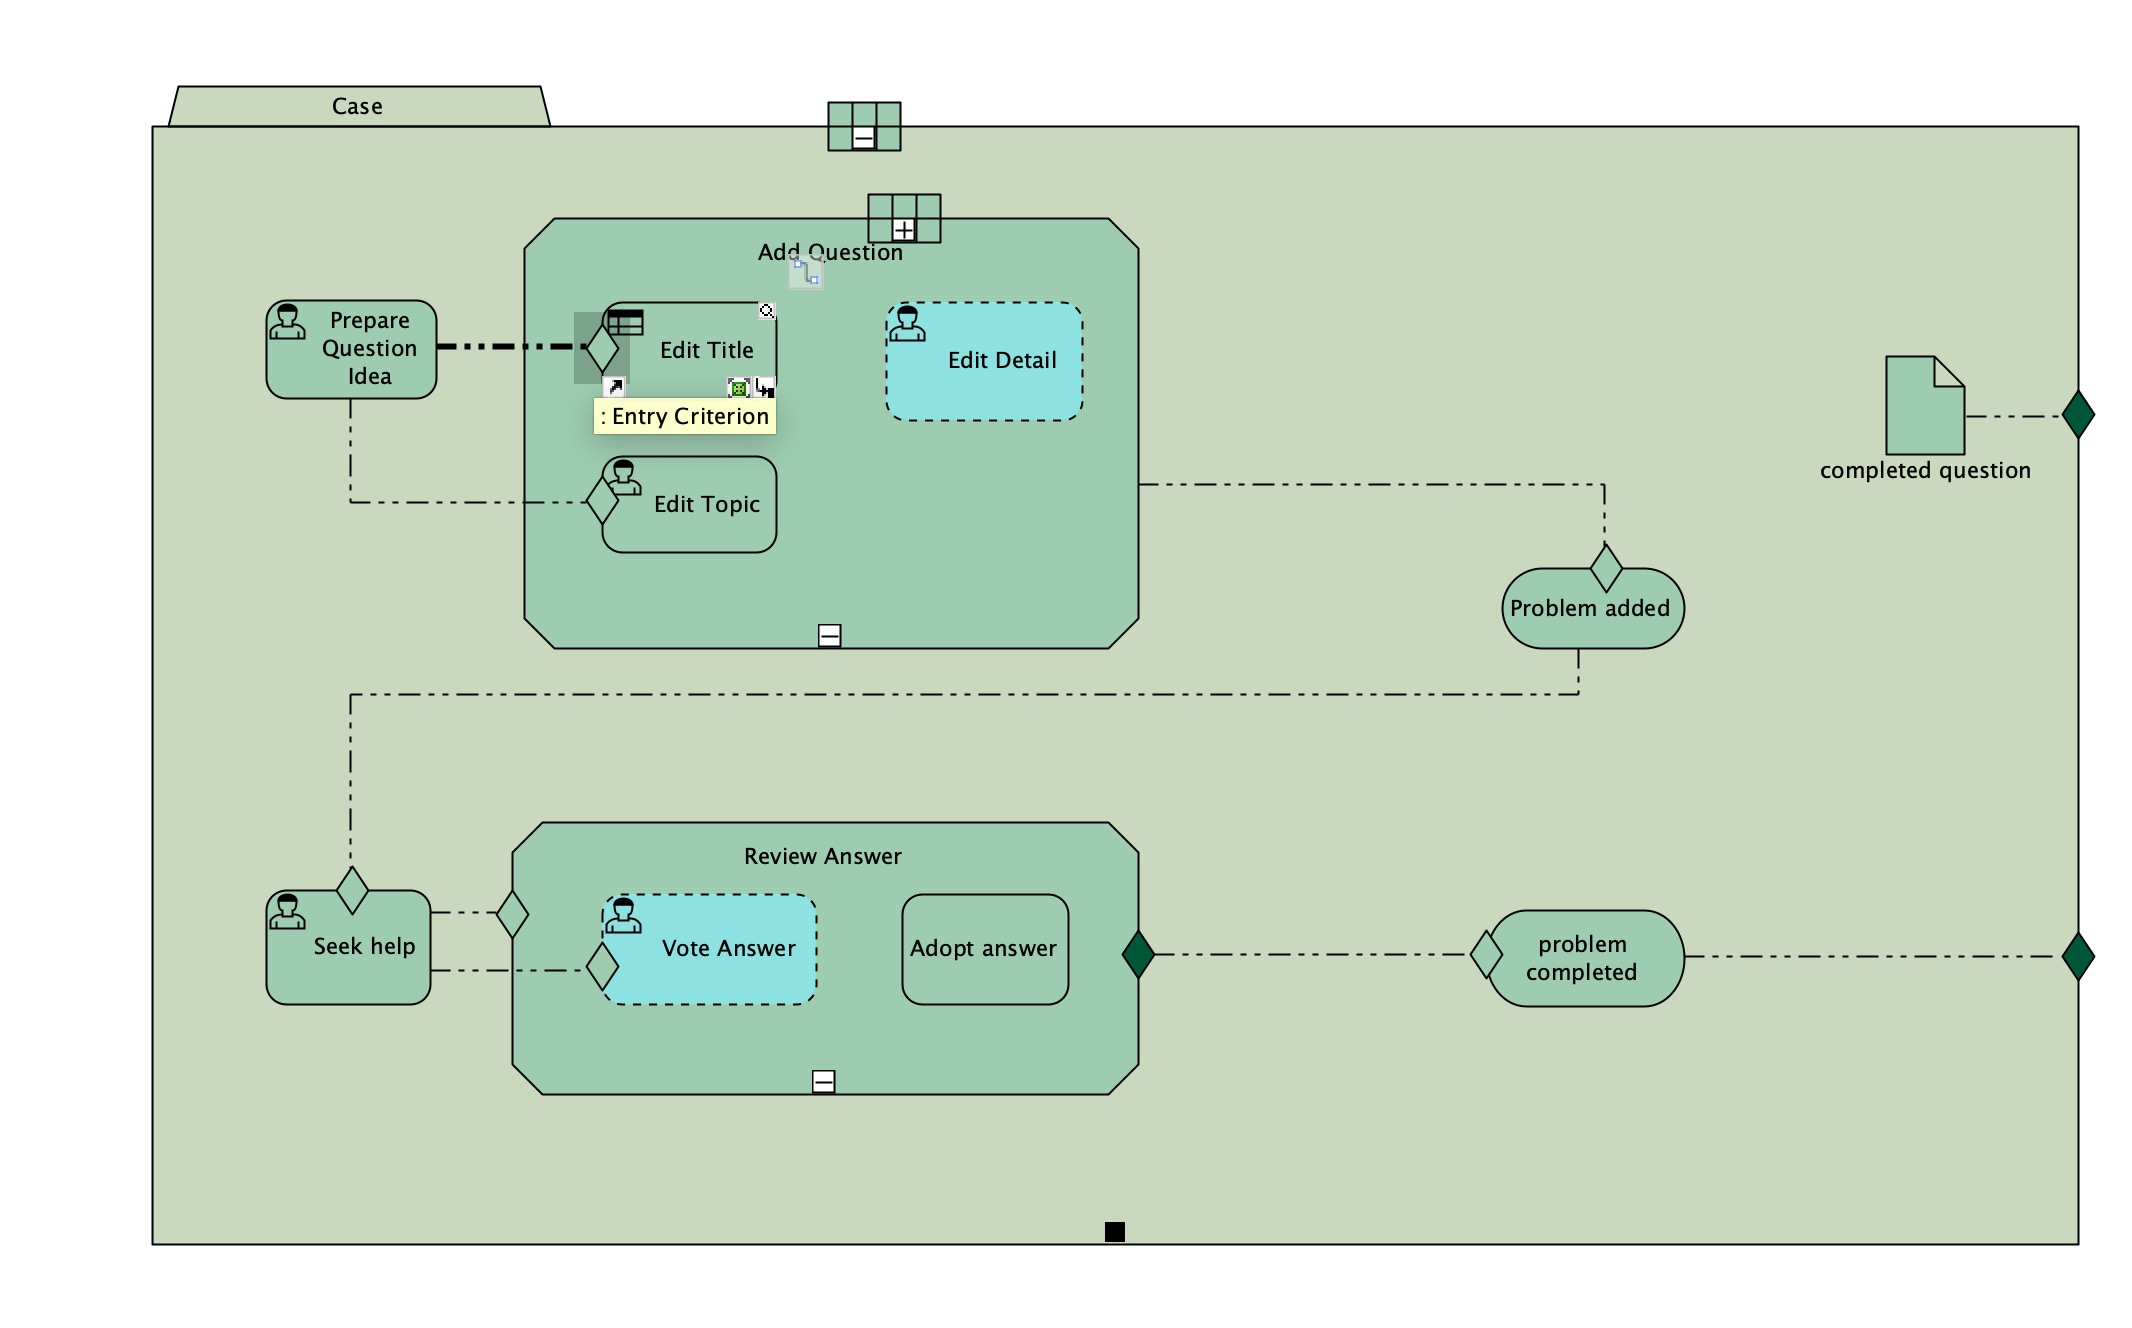
\includegraphics[width=1.0\textwidth]{figure/mwzh/cmmnmodel} %插入图片,[]中设置图片大小,{}中是图片文件名
		\caption{Q\&A Service CMMN Model} %最终文档中希望显示的图片标题
		\label{qaservice} %用于文内引用的标签
    \end{figure}   
    
    %pengmuzhe
	\noindent 
\textbf{Message Processing Service BPMN Model and XML}

\begin{figure}
  \centering
  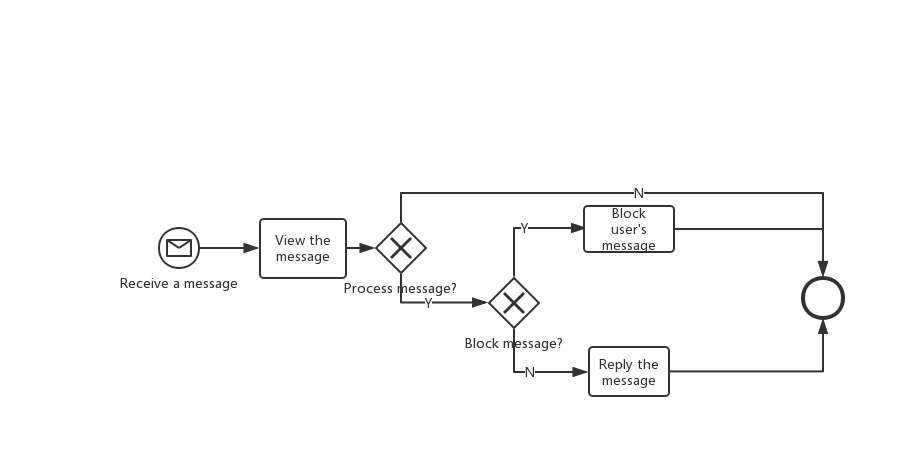
\includegraphics[width=1\textwidth]{figure/pmz/MessageManagement.png}
  \caption{Message Management}
\end{figure}
\begin{lstlisting}[language={XML}]]
<bpmn:process id="Process_1" isExecutable="true">
	<bpmn:startEvent id="StartEvent">
        <bpmn:outgoing>SequenceFlow_1</bpmn:outgoing>
        <bpmn:messageEventDefinition/>
    </bpmn:startEvent>
    <bpmn:sequenceFlow id="SequenceFlow_1" sourceRef="StartEvent" targetRef="Task_1" />
    <bpmn:task id="Task_1" name="View the message">
        <bpmn:incoming>SequenceFlow_1</bpmn:incoming>
        <bpmn:outgoing>SequenceFlow_2</bpmn:outgoing>
    </bpmn:task>
    <bpmn:sequenceFlow id="SequenceFlow_2" sourceRef="Task_1" targetRef="ExclusiveGateway_1" />
    <bpmn:exclusiveGateway id="ExclusiveGateway_1" name="Process message?">
        <bpmn:incoming>SequenceFlow_2</bpmn:incoming>
        <bpmn:outgoing>SequenceFlow_3</bpmn:outgoing>
        <bpmn:outgoing>SequenceFlow_4</bpmn:outgoing>
    </bpmn:exclusiveGateway>
    <bpmn:sequenceFlow id="SequenceFlow_3" sourceRef="ExclusiveGateway_1" targetRef="EndEvent"/>
        <bpmn:conditionExpression 
        xsi:type="bpmn:tFormalExpression">N</bpmn:conditionExpression>
    </bpmn:sequenceFlow>
     <bpmn:sequenceFlow id="SequenceFlow_4" sourceRef="ExclusiveGateway_1"
    targetRef="ExclusiveGateway_2" />
        <bpmn:conditionExpression 
        xsi:type="bpmn:tFormalExpression">Y</bpmn:conditionExpression>
    </bpmn:sequenceFlow>
     <bpmn:exclusiveGateway id="ExclusiveGateway_2" name="Block message?">
        <bpmn:incoming>SequenceFlow_4</bpmn:incoming>
        <bpmn:outgoing>SequenceFlow_5</bpmn:outgoing>
        <bpmn:outgoing>SequenceFlow_6</bpmn:outgoing>
    </bpmn:exclusiveGateway>
    <bpmn:sequenceFlow id="SequenceFlow_5" sourceRef="ExclusiveGateway_2" targetRef="Task_2" />
        <bpmn:conditionExpression 
        xsi:type="bpmn:tFormalExpression">Y</bpmn:conditionExpression>
    </bpmn:sequenceFlow>
    <bpmn:sequenceFlow id="SequenceFlow_6" sourceRef="ExclusiveGateway_2" targetRef="Task_3" />
        <bpmn:conditionExpression 
        xsi:type="bpmn:tFormalExpression">N</bpmn:conditionExpression>
    </bpmn:sequenceFlow>
    <bpmn:task id="Task_2" name="Block user's message">
        <bpmn:incoming>SequenceFlow_5</bpmn:incoming>
        <bpmn:outgoing>SequenceFlow_7</bpmn:outgoing>
    </bpmn:task>
    <bpmn:task id="Task_3" name="Reply the message">
        <bpmn:incoming>SequenceFlow_6</bpmn:incoming>
        <bpmn:outgoing>SequenceFlow_8</bpmn:outgoing>
    </bpmn:task>
    <bpmn:sequenceFlow id="SequenceFlow_7" sourceRef="Task_2" targetRef="EndEvent" />
    <bpmn:sequenceFlow id="SequenceFlow_8" sourceRef="Task_3" targetRef="EndEvent" />
    <bpmn:endEvent id="EndEvent">
        <bpmn:ingoing>SequenceFlow_3</bpmn:ingoing>
        <bpmn:ingoing>SequenceFlow_7</bpmn:ingoing>
        <bpmn:ingoing>SequenceFlow_8</bpmn:ingoing>
    </bpmn:endEvent> 
</bpmn:process>
\end{lstlisting}
\textbf{Issue Updates Service BPMN Model and XML}
\begin{figure}
  \centering
  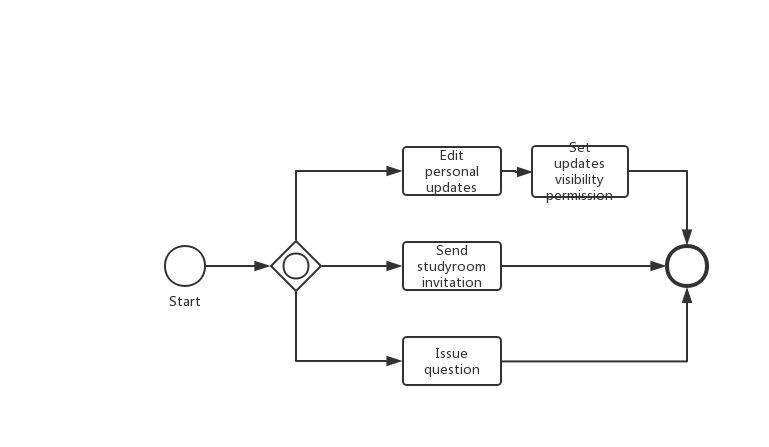
\includegraphics[width=1\textwidth]{figure/pmz/UpdatesIssueManagement.png}
  \caption{Updates Issue Management}
\end{figure}
\begin{lstlisting}[language={XML}]
<bpmn:process id="Process_3" isExecutable="true">
	<bpmn:startEvent id="StartEvent">
        <bpmn:outgoing>SequenceFlow_1</bpmn:outgoing>
    </bpmn:startEvent>
    <bpmn:sequenceFlow id="SequenceFlow_1" sourceRef="StartEvent" targetRef="InclusiveGateway" />
    <bpmn:inclusiveGateway id="InclusiveGateway">
        <bpmn:incoming>SequenceFlow_1</bpmn:incoming>
        <bpmn:outgoing>SequenceFlow_2</bpmn:outgoing>
        <bpmn:outgoing>SequenceFlow_3</bpmn:outgoing>
        <bpmn:outgoing>SequenceFlow_4</bpmn:outgoing>
    </bpmn:inclusiveGateway>
    <bpmn:sequenceFlow id="SequenceFlow_2" sourceRef="InclusiveGateway" targetRef="Task_1" />
    <bpmn:sequenceFlow id="SequenceFlow_3" sourceRef="InclusiveGateway" targetRef="Task_2" />
    <bpmn:sequenceFlow id="SequenceFlow_4" sourceRef="InclusiveGateway" targetRef="Task_3" />
    <bpmn:task id="Task_1" name="Edit Personal updates">
    	<bpmn:ingoing>SequenceFlow_2</bpmn:ingoing>
    	<bpmn:outgoing>SequenceFlow_5</bpmn:outgoing>
    </bpmn:task>
    <bpmn:task id="Task_2" name="Send studyroom invitation">
    	<bpmn:ingoing>SequenceFlow_3</bpmn:ingoing>
    	<bpmn:outgoing>SequenceFlow_6</bpmn:outgoing>
    </bpmn:task>
    <bpmn:task id="Task_3" name="Issue question">
    	<bpmn:ingoing>SequenceFlow_4</bpmn:ingoing>
    	<bpmn:outgoing>SequenceFlow_7</bpmn:outgoing>
    </bpmn:task>
    <bpmn:sequenceFlow id="SequenceFlow_5" sourceRef="Task_1" targetRef="Task_4" />
    <bpmn:sequenceFlow id="SequenceFlow_6" sourceRef="Task_2" targetRef="EndEvent" />
    <bpmn:sequenceFlow id="SequenceFlow_7" sourceRef="Task_3" targetRef="EndEvent" />
    <bpmn:task id="Task_4" name="Set updates visibility permission">
    	<bpmn:ingoing>SequenceFlow_5</bpmn:ingoing>
    	<bpmn:outgoing>EndEvent</bpmn:outgoing>
    </bpmn:task>
    <bpmn:sequenceFlow id="SequenceFlow_8" sourceRef="Task_4" targetRef="EndEvent" />
    <bpmn:endEvent id="StartEvent">
        <bpmn:ingoing>SequenceFlow_6</bpmn:ingoing>
        <bpmn:ingoing>SequenceFlow_7</bpmn:ingoing>
        <bpmn:ingoing>SequenceFlow_8</bpmn:ingoing>
    </bpmn:endEvent>
</bpmn:process>
\end{lstlisting}
\textbf{Search Service BPMN Model and XML}
\begin{figure}
  \centering
  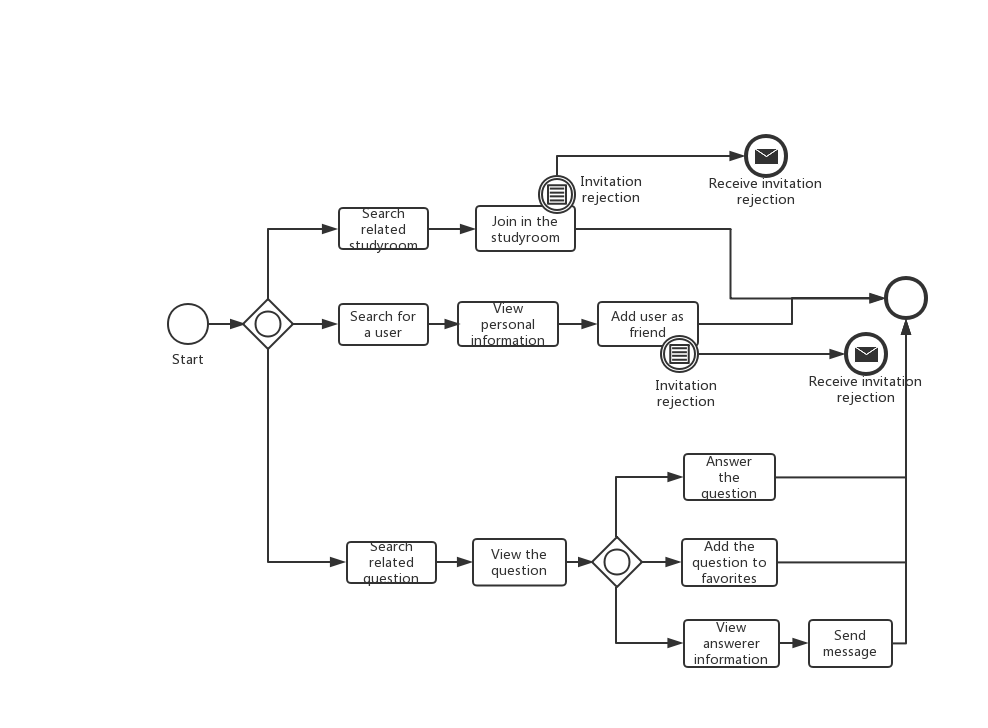
\includegraphics[width=1\textwidth]{figure/pmz/SearchManagement.png}
  \caption{Search Management}
\end{figure}
\begin{lstlisting}[language={XML}]]
<bpmn:process id="Process_2" isExecutable="true">
	<bpmn:startEvent id="StartEvent">
        <bpmn:outgoing>SequenceFlow_1</bpmn:outgoing>
    </bpmn:startEvent>
    <bpmn:sequenceFlow id="SequenceFlow_1" sourceRef="StartEvent" targetRef="InclusiveGateway_1" />
    <bpmn:inclusiveGateway id="InclusiveGateway_1">
        <bpmn:incoming>SequenceFlow_1</bpmn:incoming>
        <bpmn:outgoing>SequenceFlow_2</bpmn:outgoing>
        <bpmn:outgoing>SequenceFlow_3</bpmn:outgoing>
        <bpmn:outgoing>SequenceFlow_4</bpmn:outgoing>
    </bpmn:inclusiveGateway>
    <bpmn:sequenceFlow id="SequenceFlow_2" sourceRef="InclusiveGateway_1" targetRef="Task_1" />
    <bpmn:sequenceFlow id="SequenceFlow_3" sourceRef="InclusiveGateway_1" targetRef="Task_2" />
    <bpmn:sequenceFlow id="SequenceFlow_4" sourceRef="InclusiveGateway_1" targetRef="Task_3" />
    <bpmn:task id="Task_1" name="Search related studyroom">
        <bpmn:incoming>SequenceFlow_2</bpmn:incoming>
        <bpmn:outgoing>SequenceFlow_5</bpmn:outgoing>
    </bpmn:task>
    <bpmn:task id="Task_2" name="Search for a user">
        <bpmn:incoming>SequenceFlow_3</bpmn:incoming>
        <bpmn:outgoing>SequenceFlow_6</bpmn:outgoing>
    </bpmn:task>
    <bpmn:task id="Task_3" name="Search related question">
        <bpmn:incoming>SequenceFlow_4</bpmn:incoming>
        <bpmn:outgoing>SequenceFlow_7</bpmn:outgoing>
    </bpmn:task>
    <bpmn:sequenceFlow id="SequenceFlow_5" sourceRef="Task_1" targetRef="Task_4" />
    <bpmn:sequenceFlow id="SequenceFlow_6" sourceRef="Task_2" targetRef="Task_5" />
    <bpmn:sequenceFlow id="SequenceFlow_7" sourceRef="Task_3" targetRef="Task_5" />
    <bpmn:task id="Task_4" name="Join in the studyroom">
        <bpmn:incoming>SequenceFlow_5</bpmn:incoming>
        <bpmn:outgoing>SequenceFlow_9</bpmn:outgoing>
    </bpmn:task>
    <bpmn:task id="Task_5" name="View personal information">
        <bpmn:incoming>SequenceFlow_6</bpmn:incoming>
        <bpmn:outgoing>SequenceFlow_10</bpmn:outgoing>
    </bpmn:task>
    <bpmn:task id="Task_6" name="View the question">
        <bpmn:incoming>SequenceFlow_7</bpmn:incoming>
        <bpmn:outgoing>SequenceFlow_11</bpmn:outgoing>
    </bpmn:task>
    <bpmn:sequenceFlow id="SequenceFlow_9" sourceRef="Task_4" targetRef="EndEvent_3" />
    <bpmn:sequenceFlow id="SequenceFlow_10" sourceRef="Task_5" targetRef="Task_7" />
    <bpmn:sequenceFlow id="SequenceFlow_11" sourceRef="Task_6" targetRef="InclusiveGateway_2" />
    <bpmn:boundaryEvent id="BoundaryEvent_1" name="Invitation rejection" attachedToRef="Task_4">
        <bpmn:outgoing>SequenceFlow_8</bpmn:outgoing>
        <bpmn:conditionalEventDefinition />
    </bpmn:boundaryEvent>
    <bpmn:sequenceFlow id="SequenceFlow_8" sourceRef="BoundaryEvent_1" targetRef="EndEvent_1" />
    <bpmn:endEvent id="EndEvent_1" name="Receive invitation rejection">
        <bpmn:ingoing>SequenceFlow_8</bpmn:ingoing>
        <bpmn:messageEventDefinition/>
    </bpmn:endEvent>
    <bpmn:sequenceFlow id="SequenceFlow_12" sourceRef="InclusiveGateway_2" targetRef="Task_8" />
    <bpmn:sequenceFlow id="SequenceFlow_13" sourceRef="InclusiveGateway_2" targetRef="Task_9" />
    <bpmn:sequenceFlow id="SequenceFlow_14" sourceRef="InclusiveGateway_2" targetRef="Task_10" />
    <bpmn:sequenceFlow id="SequenceFlow_15" sourceRef="Task_7" targetRef="EndEvent_3" />
    <bpmn:task id="Task_7" name="Add user as friend">
        <bpmn:incoming>SequenceFlow_10</bpmn:incoming>
        <bpmn:outgoing>SequenceFlow_15</bpmn:outgoing>
    </bpmn:task>
    <bpmn:task id="Task_8" name="Answer the question">
        <bpmn:incoming>SequenceFlow_12</bpmn:incoming>
        <bpmn:outgoing>SequenceFlow_17</bpmn:outgoing>
    </bpmn:task>
    <bpmn:task id="Task_9" name="Add the question to favorites">
        <bpmn:incoming>SequenceFlow_13</bpmn:incoming>
        <bpmn:outgoing>SequenceFlow_18</bpmn:outgoing>
    </bpmn:task>
    <bpmn:task id="Task_10" name="View answerer's information">
        <bpmn:incoming>SequenceFlow_14</bpmn:incoming>
        <bpmn:outgoing>SequenceFlow_19</bpmn:outgoing>
    </bpmn:task>
    <bpmn:boundaryEvent id="BoundaryEvent_2" name="Invitation rejection" attachedToRef="Task_7">
        <bpmn:outgoing>SequenceFlow_16</bpmn:outgoing>
        <bpmn:conditionalEventDefinition />
    </bpmn:boundaryEvent>
    <bpmn:sequenceFlow id="SequenceFlow_16" sourceRef="BoundaryEvent_2" targetRef="EndEvent_2" />
    <bpmn:endEvent id="EndEvent_2" name="Receive invitation rejection">
        <bpmn:ingoing>SequenceFlow_16</bpmn:ingoing>
        <bpmn:messageEventDefinition/>
    </bpmn:endEvent>
    <bpmn:sequenceFlow id="SequenceFlow_17" sourceRef="Task_8" targetRef="EndEvent_3" />
    <bpmn:sequenceFlow id="SequenceFlow_18" sourceRef="Task_9" targetRef="EndEvent_3" />
    <bpmn:sequenceFlow id="SequenceFlow_19" sourceRef="Task_10" targetRef="Task_11" />
    <bpmn:task id="Task_11" name="Send message">
        <bpmn:incoming>SequenceFlow_14</bpmn:incoming>
        <bpmn:outgoing>SequenceFlow_20</bpmn:outgoing>
    </bpmn:task>
    <bpmn:sequenceFlow id="SequenceFlow_20" sourceRef="Task_11" targetRef="EndEvent_3" />
    <bpmn:endEvent id="EndEvent_3">
        <bpmn:ingoing>SequenceFlow_9</bpmn:outgoing>
        <bpmn:ingoing>SequenceFlow_15</bpmn:outgoing>
        <bpmn:ingoing>SequenceFlow_17</bpmn:outgoing>
        <bpmn:ingoing>SequenceFlow_18</bpmn:outgoing>
        <bpmn:ingoing>SequenceFlow_20</bpmn:outgoing>
    </bpmn:endEvent>
</bpmn:process>
\end{lstlisting}
\textbf{Message Replying Service CMMN Model and XML}
\begin{figure}
  \centering
  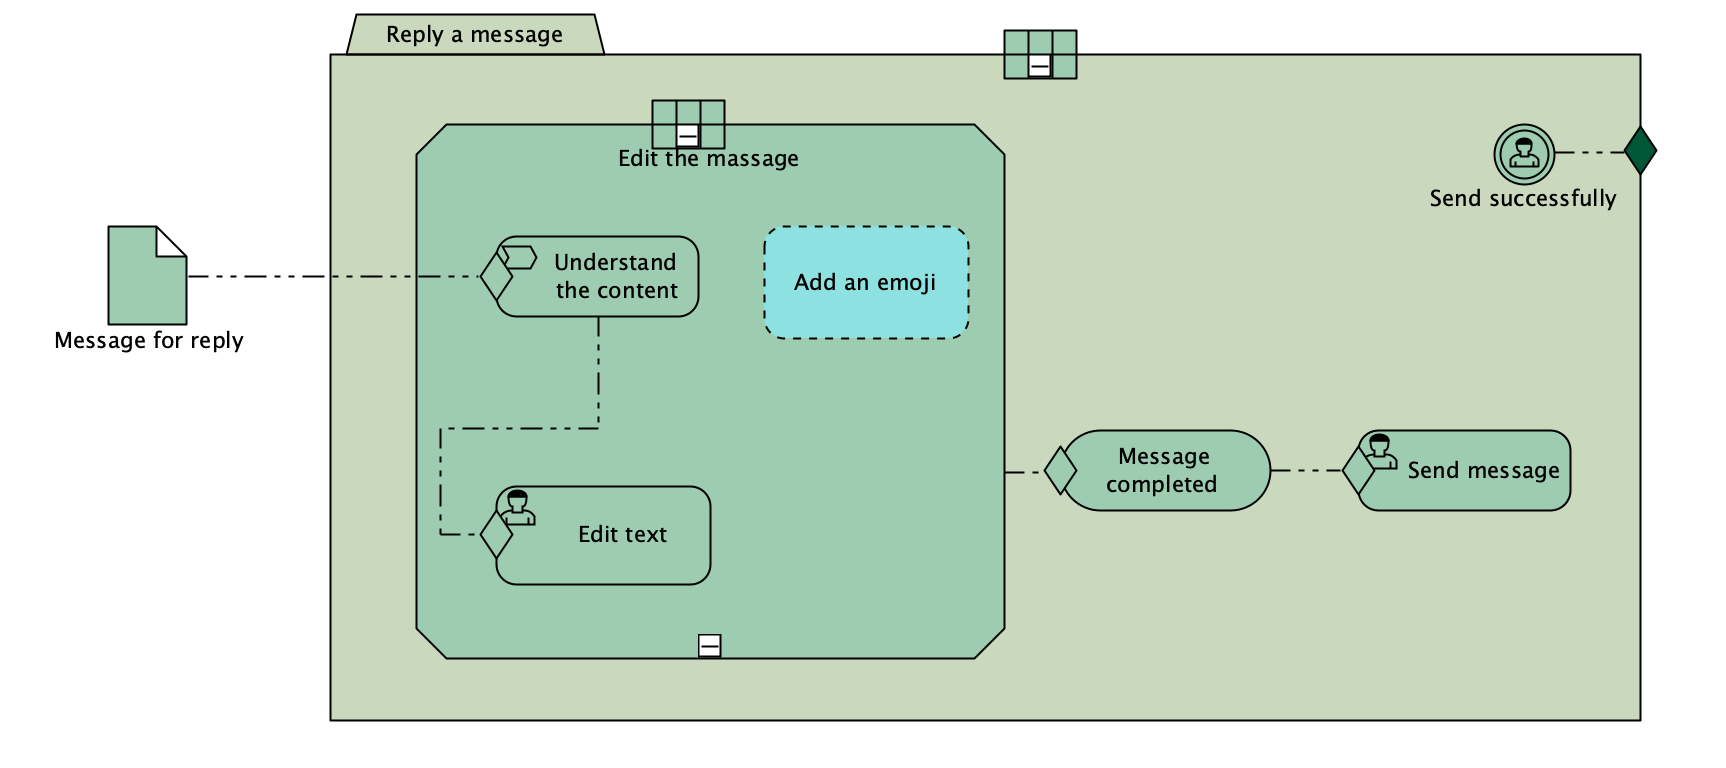
\includegraphics[width=1\textwidth]{figure/pmz/interactioncmmn}
  \caption{Reply a Message}
\end{figure}
	
	
    %heyueyue
    \textbf{Login Management Service BPMN Model and XML}\\

    \begin{figure}
       \centering %图片居中
       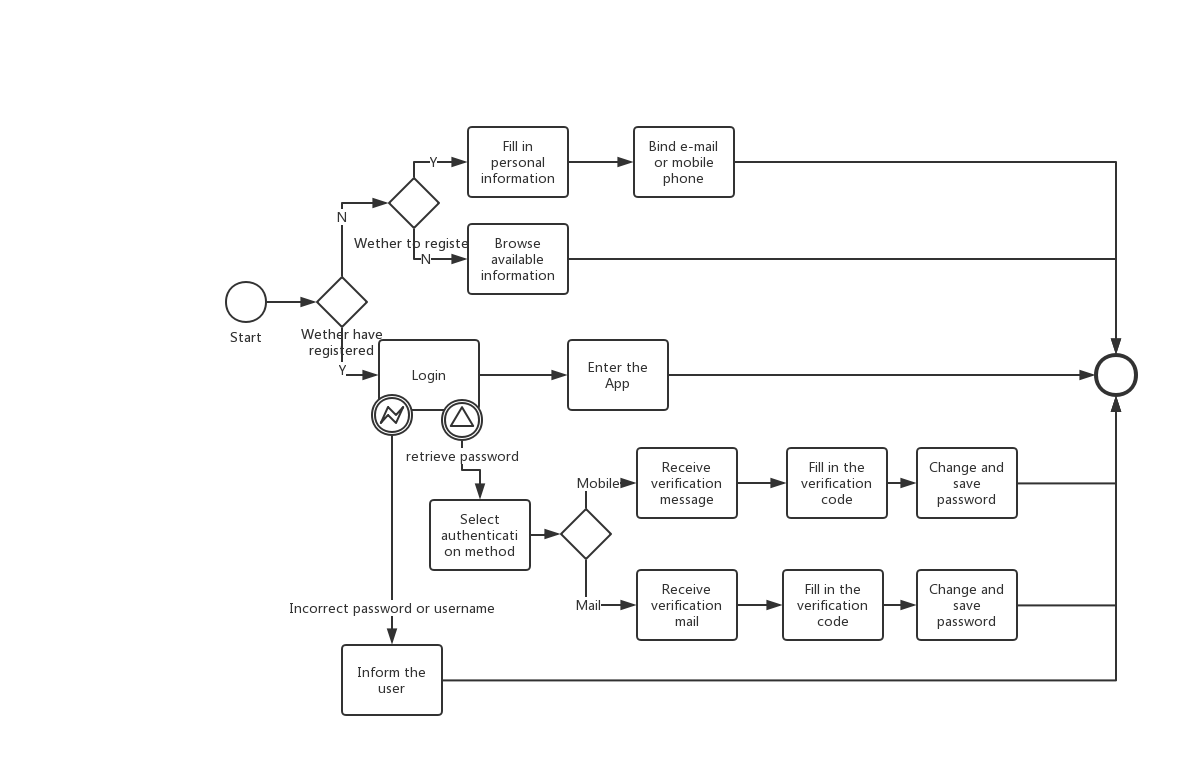
\includegraphics[width=1.0\textwidth]{figure/hyy/loginmanagement} %插入图片,[]中设置图片大小,{}中是图片文件名
       \caption{Login Service} %最终文档中希望显示的图片标题
       \label{Login Service} %用于文内引用的标签
   \end{figure}

    \noindent 
    \begin{lstlisting}[language={XML}]
        <bpmn:process id="Process_3" isExecutable="true">
	<bpmn:task id="Task_1" name="Fill in personal information">
		<bpmn:incoming>SequenceFlow_3</bpmn:incoming>
		<bpmn:outgoing>SequenceFlow_4</bpmn:outgoing>
	</bpmn:task>
	<bpmn:startEvent id="StartEvent">
		<bpmn:outgoing>SequenceFlow_1</bpmn:outgoing>
	</bpmn:startEvent>
	<bpmn:sequenceFlow id="SequenceFlow_1" sourceRef="StartEvent"
		targetRef="ExclusiveGateway_1" />
	<bpmn:sequenceFlow id="SequenceFlow_2" sourceRef="ExclusiveGateway_1"
		targetRef="ExclusiveGateway_2" >
	<bpmn:conditionExpression
		xsi:type="bpmn:tFormalExpression">N</bpmn:conditionExpression>
	</bpmn:sequenceFlow>
	<bpmn:exclusiveGateway id="ExclusiveGateway_1" name="Wether to register">
		<bpmn:incoming>SequenceFlow_1</bpmn:incoming>
		<bpmn:outgoing>SequenceFlow_2</bpmn:outgoing>
		<bpmn:outgoing>SequenceFlow_8</bpmn:outgoing>
	</bpmn:exclusiveGateway>
	<bpmn:sequenceFlow id="SequenceFlow_4" sourceRef="Task_1"
		targetRef="Task_2" />
	<bpmn:exclusiveGateway id="ExclusiveGateway_2" name="Wether have registered">
		<bpmn:incoming>SequenceFlow_2</bpmn:incoming>
		<bpmn:outgoing>SequenceFlow_3</bpmn:outgoing>
		<bpmn:outgoing>SequenceFlow_6</bpmn:outgoing>
	</bpmn:exclusiveGateway>
	<bpmn:sequenceFlow id="SequenceFlow_3" sourceRef="ExclusiveGateway_2"
		targetRef="Task_1" >
		<bpmn:conditionExpression
			xsi:type="bpmn:tFormalExpression">Y</bpmn:conditionExpression>
	</bpmn:sequenceFlow>
	<bpmn:task id="Task_2" name="Bind e-mail or mobile phone">
		<bpmn:incoming>SequenceFlow_4</bpmn:incoming>
		<bpmn:outgoing>SequenceFlow_5</bpmn:outgoing>
	</bpmn:task>
	<bpmn:sequenceFlow id="SequenceFlow_5" sourceRef="Task_2"
		targetRef="EndEvent"/>
	<bpmn:endEvent id="EndEvent">
		<bpmn:incoming>SequenceFlow_5</bpmn:incoming>
		<bpmn:incoming>SequenceFlow_7</bpmn:incoming>
		<bpmn:incoming>SequenceFlow_12</bpmn:incoming>
		<bpmn:incoming>SequenceFlow_17</bpmn:incoming>
		<bpmn:incoming>SequenceFlow_21</bpmn:incoming>
		<bpmn:incoming>SequenceFlow_22</bpmn:incoming>
	</bpmn:endEvent>
	<bpmn:sequenceFlow id="SequenceFlow_6" sourceRef="ExclusiveGateway_2"
		targetRef="Task_3">
		<bpmn:conditionExpression
			xsi:type="bpmn:tFormalExpression">N</bpmn:conditionExpression>
	</bpmn:sequenceFlow>
	<bpmn:task id="Task_3" name="Remind users">
		<bpmn:incoming>SequenceFlow_6</bpmn:incoming>
		<bpmn:outgoing>SequenceFlow_7</bpmn:outgoing>
	</bpmn:task>
	<bpmn:sequenceFlow id="SequenceFlow_7" sourceRef="Task_3"
		targetRef="EndEvent"/>
	<bpmn:sequenceFlow id="SequenceFlow_8" sourceRef="ExclusiveGateway_1"
		targetRef="Task_4">
		<bpmn:conditionExpression
			xsi:type="bpmn:tFormalExpression">Y</bpmn:conditionExpression>
	</bpmn:sequenceFlow>
	<bpmn:task id="Task_4" name="Login">
		<bpmn:incoming>SequenceFlow_8</bpmn:incoming>
		<bpmn:outgoing>SequenceFlow_11</bpmn:outgoing>
	</bpmn:task>
	<bpmn:sequenceFlow id="SequenceFlow_11" sourceRef="Task_4"
		targetRef="Task_5" />
	<bpmn:task id="Task_5" name="Enter the App">
		<bpmn:incoming>SequenceFlow_11</bpmn:incoming>
		<bpmn:outgoing>SequenceFlow_12</bpmn:outgoing>
	</bpmn:task>
	<bpmn:sequenceFlow id="SequenceFlow_12" sourceRef="Task_5"
		targetRef="EndEvent" />
	<bpmn:boundaryEvent id="BoundaryEvent_1" attachedToRef="Task_4">
		<bpmn:outgoing>SequenceFlow_9</bpmn:outgoing>
		<bpmn:errorEventDefinition />
	</bpmn:boundaryEvent>
	<bpmn:sequenceFlow id="SequenceFlow_9" sourceRef="BoundaryEvent_1"
		targetRef="Task_6" >
		<bpmn:conditionExpression
			xsi:type="bpmn:tFormalExpression">Incorrect password or username</bpmn:conditionExpression>
	</bpmn:sequenceFlow>
	<bpmn:task id="Task_6" name="Inform the user">
		<bpmn:incoming>SequenceFlow_9</bpmn:incoming>
		<bpmn:outgoing>SequenceFlow_22</bpmn:outgoing>
	</bpmn:task>
	<bpmn:sequenceFlow id="SequenceFlow_22" sourceRef="Task_6"
		targetRef="EndEvent" />
	<bpmn:boundaryEvent id="BoundaryEvent_2" attachedToRef="Task_4">
		<bpmn:outgoing>SequenceFlow_10</bpmn:outgoing>
		<bpmn:signalEventDefinition />
	</bpmn:boundaryEvent>
	<bpmn:sequenceFlow id="SequenceFlow_10" sourceRef="BoundaryEvent_2"
		targetRef="Task_7" >
		<bpmn:conditionExpression
			xsi:type="bpmn:tFormalExpression">retrieve password</bpmn:conditionExpression>
	</bpmn:sequenceFlow>
	<bpmn:task id="Task_7" name="Select authentication method">
		<bpmn:incoming>SequenceFlow_10</bpmn:incoming>
		<bpmn:outgoing>SequenceFlow_13</bpmn:outgoing>
	</bpmn:task>
	<bpmn:sequenceFlow id="SequenceFlow_13" sourceRef="Task_7"
		targetRef="ExclusiveGateway_3" />
	<bpmn:exclusiveGateway id="ExclusiveGateway_3">
		<bpmn:incoming>SequenceFlow_13</bpmn:incoming>
		<bpmn:outgoing>SequenceFlow_14</bpmn:outgoing>
		<bpmn:outgoing>SequenceFlow_18</bpmn:outgoing>
	</bpmn:exclusiveGateway>
	<bpmn:sequenceFlow id="SequenceFlow_14" sourceRef="ExclusiveGateway_3"
		targetRef="Task_8" >
		<bpmn:conditionExpression
			xsi:type="bpmn:tFormalExpression">Mobile</bpmn:conditionExpression>
	</bpmn:sequenceFlow>
	<bpmn:task id="Task_8" name="Receive verification message">
		<bpmn:incoming>SequenceFlow_14</bpmn:incoming>
		<bpmn:outgoing>SequenceFlow_15</bpmn:outgoing>
	</bpmn:task>
	<bpmn:sequenceFlow id="SequenceFlow_15" sourceRef="Task_8"
		targetRef="Task_9" />
	<bpmn:task id="Task_9" name="Fill in the verification code">
		<bpmn:incoming>SequenceFlow_15</bpmn:incoming>
		<bpmn:outgoing>SequenceFlow_16</bpmn:outgoing>
	</bpmn:task>
	<bpmn:sequenceFlow id="SequenceFlow_16" sourceRef="Task_9"
		targetRef="Task_10" />
	<bpmn:task id="Task_10" name="Change and save password">
		<bpmn:incoming>SequenceFlow_16</bpmn:incoming>
		<bpmn:outgoing>SequenceFlow_17</bpmn:outgoing>
	</bpmn:task>
	<bpmn:sequenceFlow id="SequenceFlow_17" sourceRef="Task_10"
		targetRef="EndEvent" />
	<bpmn:sequenceFlow id="SequenceFlow_18" sourceRef="ExclusiveGateway_3"
		targetRef="Task_11" >
		<bpmn:conditionExpression       xsi:type="bpmn:tFormalExpression">Mail</bpmn:conditionExpression>
	</bpmn:sequenceFlow>
	<bpmn:task id="Task_11" name="Receive verification mail">
		<bpmn:incoming>SequenceFlow_18</bpmn:incoming>
		<bpmn:outgoing>SequenceFlow_19</bpmn:outgoing>
	</bpmn:task>
	<bpmn:sequenceFlow id="SequenceFlow_19" sourceRef="Task_11"
		targetRef="Task_12" />
	<bpmn:task id="Task_12" name="Fill in the verification code">
		<bpmn:incoming>SequenceFlow_19</bpmn:incoming>
		<bpmn:outgoing>SequenceFlow_20</bpmn:outgoing>
	</bpmn:task>
	<bpmn:sequenceFlow id="SequenceFlow_20" sourceRef="Task_12"
		targetRef="Task_13" />
	<bpmn:task id="Task_13" name="Change and save password">
		<bpmn:incoming>SequenceFlow_20</bpmn:incoming>
		<bpmn:outgoing>SequenceFlow_21</bpmn:outgoing>
	</bpmn:task>
	<bpmn:sequenceFlow id="SequenceFlow_21" sourceRef="Task_13"
		targetRef="EndEvent" />
	</bpmn:process>
    
	\end{lstlisting}



    \clearpage
    \textbf{Study Plan Management Service BPMN Model and XML}\\
   \begin{figure}
       \centering %图片居中
      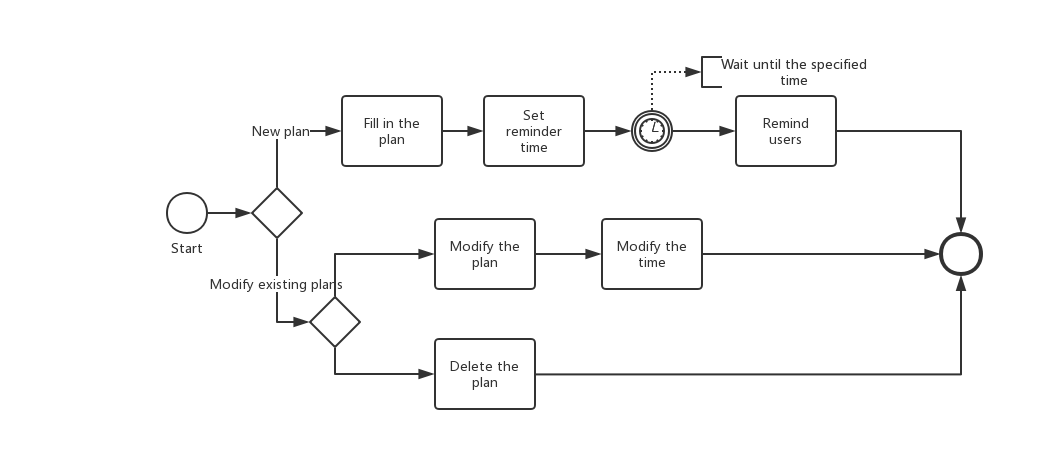
\includegraphics[width=1.0\textwidth]{figure/hyy/studyplanmanagement} %插入图片,[]中设置图片大小,{}中是图片文件名
       \caption{Study Plan Service} %最终文档中希望显示的图片标题
      % \label{Study Plan service} %用于文内引用的标签
   \end{figure}

    \begin{lstlisting}[language={XML}]
        <bpmn:process id="Process_2" isExecutable="true">
<bpmn:task id="Task_1" name="Fill in the plan">
    <bpmn:incoming>SequenceFlow_2</bpmn:incoming>
    <bpmn:outgoing>SequenceFlow_3</bpmn:outgoing>
</bpmn:task>
<bpmn:startEvent id="StartEvent">
    <bpmn:outgoing>SequenceFlow_1</bpmn:outgoing>
</bpmn:startEvent>
<bpmn:sequenceFlow id="SequenceFlow_1" sourceRef="StartEvent"
    targetRef="ExclusiveGateway_1" />
<bpmn:sequenceFlow id="SequenceFlow_2" sourceRef="ExclusiveGateway_1"
    targetRef="Task_1">
    <bpmn:conditionExpression
        xsi:type="bpmn:tFormalExpression">New plan</bpmn:conditionExpression>
</bpmn:sequenceFlow>
<bpmn:exclusiveGateway id="ExclusiveGateway_1">
    <bpmn:incoming>SequenceFlow_1</bpmn:incoming>
    <bpmn:outgoing>SequenceFlow_2</bpmn:outgoing>
    <bpmn:outgoing>SequenceFlow_7</bpmn:outgoing>
</bpmn:exclusiveGateway>
<bpmn:sequenceFlow id="SequenceFlow_3" sourceRef="Task_1"
    targetRef="Task_2" />
<bpmn:sequenceFlow id="SequenceFlow_7" sourceRef="ExclusiveGateway_1"
    targetRef="ExclusiveGateway_2">
    <bpmn:conditionExpression
        xsi:type="bpmn:tFormalExpression">Modify existing plans</bpmn:conditionExpression>
</bpmn:sequenceFlow>
<bpmn:task id="Task_2" name="Set reminder time">
    <bpmn:incoming>SequenceFlow_3</bpmn:incoming>
    <bpmn:outgoing>SequenceFlow_4</bpmn:outgoing>
</bpmn:task>
<bpmn:sequenceFlow id="SequenceFlow_4" sourceRef="Task_2"
    targetRef="IntermediateCatchEvent"/>
<bpmn:intermediateCatchEvent id="IntermediateCatchEvent">
    <bpmn:incoming>SequenceFlow_4</bpmn:incoming>
    <bpmn:outgoing>SequenceFlow_5</bpmn:outgoing>
    <bpmn:timeEventDefinition />
</bpmn:intermediateCatchEvent>
<bpmn:sequenceFlow id="SequenceFlow_5" sourceRef="IntermediateCatchEvent"
    targetRef="Task_3"/>
<bpmn:task id="Task_3" name="Remind users">
    <bpmn:incoming>SequenceFlow_5</bpmn:incoming>
    <bpmn:outgoing>SequenceFlow_6</bpmn:outgoing>
</bpmn:task>
<bpmn:sequenceFlow id="SequenceFlow_6" sourceRef="Task_3"
    targetRef="EndEvent"/>
<bpmn:endEvent id="EndEvent">
    <bpmn:incoming>SequenceFlow_6</bpmn:incoming>
    <bpmn:incoming>SequenceFlow_10</bpmn:incoming>
    <bpmn:incoming>SequenceFlow_12</bpmn:incoming>
</bpmn:endEvent>
<bpmn:exclusiveGateway id="ExclusiveGateway_2">
    <bpmn:incoming>SequenceFlow_7</bpmn:incoming>
    <bpmn:outgoing>SequenceFlow_8</bpmn:outgoing>
    <bpmn:outgoing>SequenceFlow_11</bpmn:outgoing>
</bpmn:exclusiveGateway>
<bpmn:sequenceFlow id="SequenceFlow_8" sourceRef="ExclusiveGateway_2"
    targetRef="Task_4" />
<bpmn:task id="Task_4" name="Modify the plan">
    <bpmn:incoming>SequenceFlow_8</bpmn:incoming>
    <bpmn:outgoing>SequenceFlow_9</bpmn:outgoing>
</bpmn:task>
<bpmn:sequenceFlow id="SequenceFlow_9" sourceRef="Task_4"
    targetRef="Task_5" />
<bpmn:task id="Task_5" name="Modify the time">
    <bpmn:incoming>SequenceFlow_9</bpmn:incoming>
    <bpmn:outgoing>SequenceFlow_10</bpmn:outgoing>
</bpmn:task>
<bpmn:sequenceFlow id="SequenceFlow_10" sourceRef="Task_5"
    targetRef="EndEvent" />
<bpmn:sequenceFlow id="SequenceFlow_11" sourceRef="ExclusiveGateway_2"
    targetRef="Task_6" />
<bpmn:task id="Task_6" name="Delete the plan">
    <bpmn:incoming>SequenceFlow_11</bpmn:incoming>
    <bpmn:outgoing>SequenceFlow_12</bpmn:outgoing>
</bpmn:task>
<bpmn:sequenceFlow id="SequenceFlow_12" sourceRef="Task_6"
    targetRef="EndEvent" />
<bpmn:textAnnotation id="TextAnnotation_1">
    <bpmn:text>Wait until the specified time</bpmn:text>
</bpmn:textAnnotation>
<bpmn:association id="Association_1" sourceRef="IntermediateCatchEvent"
    targetRef="TextAnnotation_1" />
</bpmn:process>
	\end{lstlisting}
	
    \clearpage
     \textbf{Personal data management Service BPMN Model and XML}\\
    \begin{figure}
        \centering %图片居中
        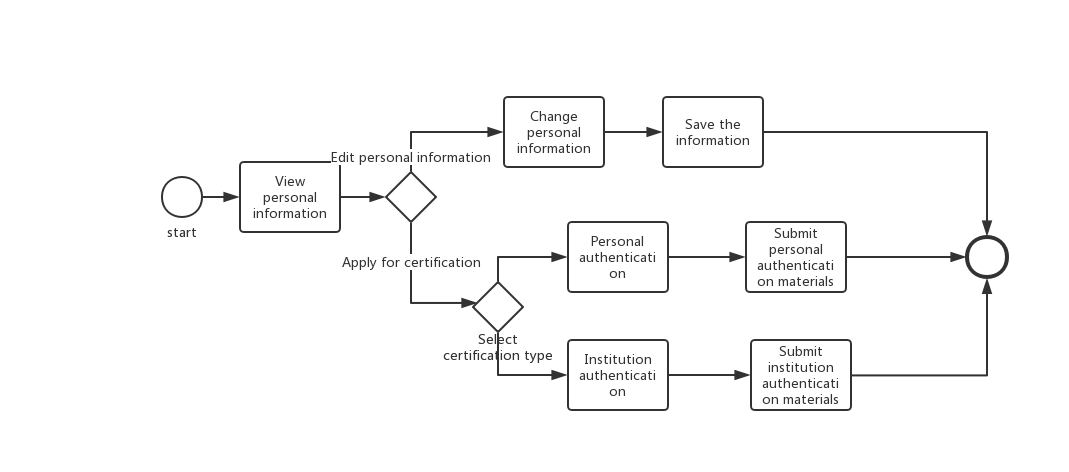
\includegraphics[width=1.0\textwidth]{figure/hyy/personaldatamanagement} %插入图片,[]中设置图片大小,{}中是图片文件名
       %\caption{Personal data management Service BPMN Model}\\
        \label{Personal data management} %用于文内引用的标签
   \end{figure}
   \begin{lstlisting}[language={XML}]
   <bpmn:process id="Process_1" isExecutable="true">
    <bpmn:task id="Task_1" name="View personal information">
        <bpmn:incoming>SequenceFlow_1</bpmn:incoming>
        <bpmn:outgoing>SequenceFlow_2</bpmn:outgoing>
    </bpmn:task>
<bpmn:startEvent id="StartEvent">
        <bpmn:outgoing>SequenceFlow_1</bpmn:outgoing>
    </bpmn:startEvent>
    <bpmn:sequenceFlow id="SequenceFlow_1" sourceRef="StartEvent"
        targetRef="Task_1" />
    <bpmn:sequenceFlow id="SequenceFlow_2" sourceRef="Task_1"
        targetRef="ExclusiveGateway_1" />
    <bpmn:exclusiveGateway id="ExclusiveGateway_1">
        <bpmn:incoming>SequenceFlow_2</bpmn:incoming>
        <bpmn:outgoing>SequenceFlow_3</bpmn:outgoing>
        <bpmn:outgoing>SequenceFlow_6</bpmn:outgoing>
    </bpmn:exclusiveGateway>
    <bpmn:task id="Task_2" name="Change personal information">
        <bpmn:incoming>SequenceFlow_3</bpmn:incoming>
        <bpmn:outgoing>SequenceFlow_4</bpmn:outgoing>
    </bpmn:task>
    <bpmn:sequenceFlow id="SequenceFlow_4" sourceRef="Task_2"
        targetRef="Task_3" />
    <bpmn:task id="Task_3" name="Save the information">
        <bpmn:incoming>SequenceFlow_4</bpmn:incoming>
        <bpmn:outgoing>SequenceFlow_5</bpmn:outgoing>
    </bpmn:task>
    <bpmn:sequenceFlow id="SequenceFlow_5" sourceRef="Task_3"
        targetRef="EndEvent" />
    <bpmn:endEvent id="EndEvent">
        <bpmn:incoming>SequenceFlow_5</bpmn:incoming>
        <bpmn:incoming>SequenceFlow_9</bpmn:incoming>
        <bpmn:incoming>SequenceFlow_12</bpmn:incoming>
    </bpmn:endEvent>
    <bpmn:sequenceFlow id="SequenceFlow_9" sourceRef="Task_5"
        targetRef="EndEvent" />
    <bpmn:sequenceFlow id="SequenceFlow_12" sourceRef="Task_7"
        targetRef="EndEvent" />
    <bpmn:sequenceFlow id="SequenceFlow_3" sourceRef="ExclusiveGateway_1"
        targetRef="Task_2">
        <bpmn:conditionExpression
            xsi:type="bpmn:tFormalExpression">Edit personal information</bpmn:conditionExpression>
    </bpmn:sequenceFlow>
    <bpmn:sequenceFlow id="SequenceFlow_6" sourceRef="ExclusiveGateway_1"
        targetRef="ExclusiveGateway_2">
        <bpmn:conditionExpression
            xsi:type="bpmn:tFormalExpression">Apply for certification</bpmn:conditionExpression>
    </bpmn:sequenceFlow>
    <bpmn:exclusiveGateway id="ExclusiveGateway_2">
        <bpmn:incoming>SequenceFlow_6</bpmn:incoming>
        <bpmn:outgoing>SequenceFlow_7</bpmn:outgoing>
        <bpmn:outgoing>SequenceFlow_10</bpmn:outgoing>
    </bpmn:exclusiveGateway>
    <bpmn:sequenceFlow id="SequenceFlow_7" sourceRef="ExclusiveGateway_2"
        targetRef="Task_4" />
    <bpmn:sequenceFlow id="SequenceFlow_10" sourceRef="ExclusiveGateway_2"
        targetRef="Task_6" />
    <bpmn:task id="Task_4" name="Personal authentication">
        <bpmn:incoming>SequenceFlow_7</bpmn:incoming>
        <bpmn:outgoing>SequenceFlow_8</bpmn:outgoing>
    </bpmn:task>
    <bpmn:task id="Task_6" name="Institution authentication">
        <bpmn:incoming>SequenceFlow_10</bpmn:incoming>
        <bpmn:outgoing>SequenceFlow_11</bpmn:outgoing>
    </bpmn:task>
    <bpmn:sequenceFlow id="SequenceFlow_8" sourceRef="Task_4"
        targetRef="Task_5" />
    <bpmn:sequenceFlow id="SequenceFlow_11" sourceRef="Task_6"
        targetRef="Task_7" />
    <bpmn:task id="Task_5" name="Submit personal authentication materials">
        <bpmn:incoming>SequenceFlow_8</bpmn:incoming>
        <bpmn:outgoing>SequenceFlow_9</bpmn:outgoing>
    </bpmn:task>
    <bpmn:task id="Task_7" name="Submit institution authentication materials">
        <bpmn:incoming>SequenceFlow_11</bpmn:incoming>
        <bpmn:outgoing>SequenceFlow_12</bpmn:outgoing>
    </bpmn:task>
</bpmn:process>
   \end{lstlisting}
    \clearpage


    \textbf{Learning Report Service CMMN Model and XML}\\
    \begin{figure}
        \centering %图片居中
        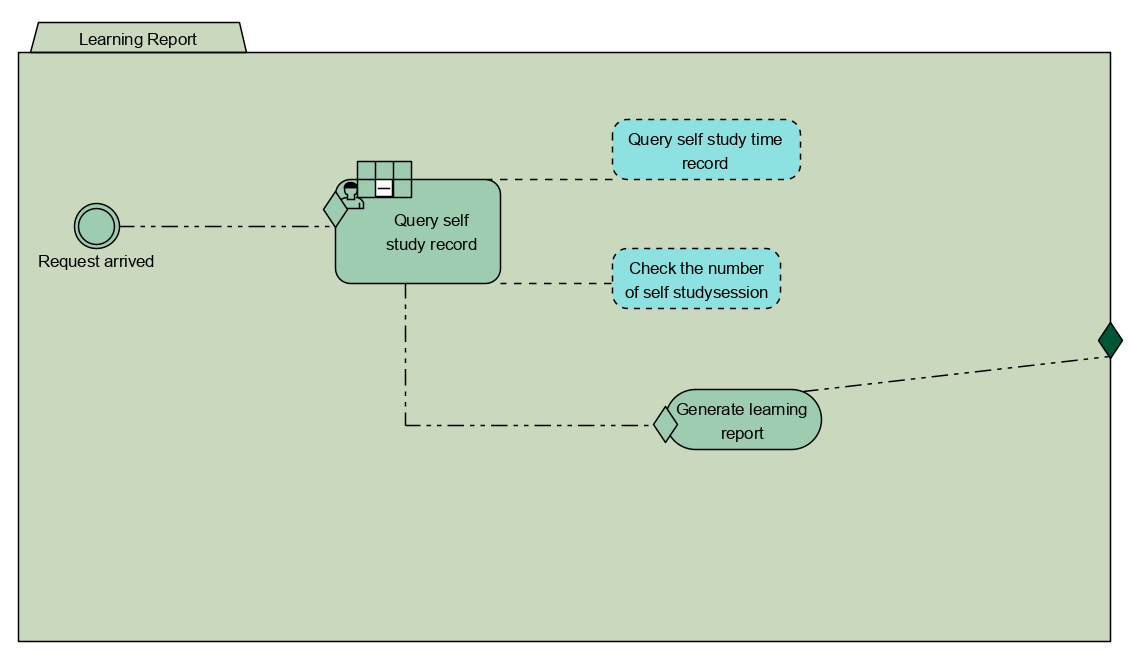
\includegraphics[width=1.0\textwidth]{figure/hyy/CMMN} %插入图片,[]中设置图片大小,{}中是图片文件名
       \caption{Learning Report Service CMMN Model} %最终文档中希望显示的图片标题
        \label{Learning Report} %用于文内引用的标签
   \end{figure}
   \begin{lstlisting}[language={XML}]
   <cmmn:case id="Case_1">
    <cmmn:casePlanModel id="CasePlanModel_1" name="Learning Report">
        <cmmn:planItem id="PlanItem_1" name="wait for request" definitionRef="TimerEventListener" />
        <cmmn:humanTask id="HumanTask_1" name="Task A">
            <cmmn:entryCriterion id="EntryCriterion_1" sentryRef="Sentry_1" />
            <cmmn:planningTable id="PlanningTable_1">
                <cmmn:discretionaryItem id="DiscretionaryItem_1" definitionRef="HumanTask_2"/>
                <cmmn:discretionaryItem id="DiscretionaryItem_2" definitionRef="HumanTask_3"/>
            </cmmn:planningTable>
        </cmmn:humanTask>
        <cmmn:sentry id="Sentry_1">
            <cmmn:planItemOnPart id="PlanItemOnPart_1" sourceRef="PlanItem_1">
                <cmmn:standardEvent>complete</cmmn:standardEvent>
            </cmmn:planItemOnPart>
        </cmmn:sentry>
        <cmmn:sentry id="Sentry_2">
            <cmmn:planItemOnPart id="PlanItemOnPart_1" sourceRef="PlanItem_1">
                <cmmn:standardEvent>complete</cmmn:standardEvent>
            </cmmn:planItemOnPart>
        </cmmn:sentry>
        <cmmn:sentry id="Sentry_3">
            <cmmn:planItemOnPart id="PlanItemOnPart_1" sourceRef="PlanItem_1">
                <cmmn:standardEvent>complete</cmmn:standardEvent>
            </cmmn:planItemOnPart>
        </cmmn:sentry>
        <cmmn:milestone id="Milestone_One" name="Milestone One">
           <cmmn:entryCriterion id="EntryCriterion_2" sentryRef="Sentry_2" />
        </cmmn:milestone>
    </cmmn:casePlanModel>
    </cmmn:case>

    \end{lstlisting}
	\clearpage
	
    %lvliting
	\noindent 
    \begin{lstlisting}[language={XML}]
        <bpmn:collaboration id="Collaboration_1">
		<bpmn:participant id="Participant_1" processRef="Process_1"/>
		<bpmn:participant id="Participant_2" processRef="Process_2"/>
		<bpmn:messageFlow id="MessageFlow_1" sourceRef="Participant_2" targetRef="Participant_1"/>
	</bpmn:collaboration>
	<bpmn:collaboration id="Collaboration_2">
		<bpmn:participant id="Participant_1" processRef="Process_1"/>
		<bpmn:participant id="Participant_2" processRef="Process_2"/>
		<bpmn:messageFlow id="MessageFlow_2" sourceRef="Participant_1" targetRef="Participant_2"/>
	</bpmn:collaboration>
	<bpmn:collaboration id="Collaboration_3">
		<bpmn:participant id="Participant_1" processRef="Process_1"/>
		<bpmn:participant id="Participant_2" processRef="Process_2"/>
		<bpmn:messageFlow id="MessageFlow_3" sourceRef="Participant_1" targetRef="Participant_2"/>
	</bpmn:collaboration>
	<bpmn:collaboration id="Collaboration_4">
		<bpmn:participant id="Participant_3" processRef="Process_3"/>
		<bpmn:participant id="Participant_2" processRef="Process_2"/>
		<bpmn:messageFlow id="MessageFlow_4" sourceRef="Participant_2" targetRef="Participant_3"/>
	</bpmn:collaboration>
	<bpmn:collaboration id="Collaboration_5">
		<bpmn:participant id="Participant_3" processRef="Process_3"/>
		<bpmn:participant id="Participant_1" processRef="Process_1"/>
		<bpmn:messageFlow id="MessageFlow_5" sourceRef="Participant_3" targetRef="Participant_1"/>
	</bpmn:collaboration>
	<bpmn:process id="Process_1" isExecutable="true">
		<bpmn:startEvent id="StartEvent_1">
	        <bpmn:outgoing>SequenceFlow_1</bpmn:outgoing>
	    </bpmn:startEvent>
		<bpmn:task id="Task_1" name="Create self-study room">
	        <bpmn:incoming>SequenceFlow_1</bpmn:incoming>
	        <bpmn:outgoing>SequenceFlow_2</bpmn:outgoing>
	    </bpmn:task>
		<bpmn:sequenceFlow id="SequenceFlow_1" sourceRef="StartEvent_1"
	        targetRef="Task_1" />
		<bpmn:exclusiveGateway id="ExclusiveGateway_1">
			<bpmn:incoming>SequenceFlow_2</bpmn:incoming>
			<bpmn:incoming>SequenceFlow_6</bpmn:incoming>
	        <bpmn:outgoing>SequenceFlow_3</bpmn:outgoing>
			<bpmn:outgoing>SequenceFlow_5</bpmn:outgoing>
		</bpmn:exclusiveGateway>
		<bpmn:sequenceFlow id="SequenceFlow_2" sourceRef="Task_1"
	        targetRef="ExclusiveGateway_1" />
		<bpmn:task id="Task_2" name="Delete self-study room">
	        <bpmn:incoming>SequenceFlow_3</bpmn:incoming>
	        <bpmn:outgoing>SequenceFlow_4</bpmn:outgoing>
	    </bpmn:task>
		<bpmn:sequenceFlow id="SequenceFlow_3" sourceRef="ExclusiveGateway_1"
			targetRef="Task_2">
			<bpmn:conditionExpression
				xsi:type="bpmn:tFormalExpression">Delete</bpmn:conditionExpression>
		</bpmn:sequenceFlow>
		<bpmn:endEvent id="EndEvent_1">
			<bpmn:incoming>SequenceFlow_4</bpmn:incoming>
		</bpmn:endEvent>
		<bpmn:sequenceFlow id="SequenceFlow_4" sourceRef="Task_2"
	        targetRef="EndEvent_1" />
		<bpmn:task id="Task_3" name="Update self-study room">
	        <bpmn:incoming>SequenceFlow_5</bpmn:incoming>
	        <bpmn:outgoing>SequenceFlow_7</bpmn:outgoing>
	    </bpmn:task>
		<bpmn:sequenceFlow id="SequenceFlow_5" sourceRef="ExclusiveGateway_1"
			targetRef="Task_3">
			<bpmn:conditionExpression
				xsi:type="bpmn:tFormalExpression">Update</bpmn:conditionExpression>
		</bpmn:sequenceFlow>
		<bpmn:task id="Task_4" name="Put self-study room online">
	        <bpmn:incoming>SequenceFlow_7</bpmn:incoming>
	        <bpmn:outgoing>SequenceFlow_8</bpmn:outgoing>
	    </bpmn:task>
		<bpmn:sequenceFlow id="SequenceFlow_7" sourceRef="Task_3"
	        targetRef="Task_4" />
		<bpmn:task id="Task_5" name="Recieve application for joining self-study room">
	        <bpmn:incoming>SequenceFlow_8</bpmn:incoming>
			<bpmn:incoming>MessageFlow_1</bpmn:incoming>
	        <bpmn:outgoing>SequenceFlow_9</bpmn:outgoing>
	    </bpmn:task>
		<bpmn:sequenceFlow id="SequenceFlow_8" sourceRef="Task_4"
	        targetRef="Task_5" />
		<bpmn:exclusiveGateway id="ExclusiveGateway_2">
			<bpmn:incoming>SequenceFlow_9</bpmn:incoming>
	        <bpmn:outgoing>SequenceFlow_10</bpmn:outgoing>
			<bpmn:outgoing>SequenceFlow_11</bpmn:outgoing>
		</bpmn:exclusiveGateway>
		<bpmn:sequenceFlow id="SequenceFlow_9" sourceRef="Task_5"
	        targetRef="ExclusiveGateway_2" />
		<bpmn:task id="Task_7" name="Allow student in the self-study room">
	        <bpmn:incoming>SequenceFlow_10</bpmn:incoming>
	        <bpmn:outgoing>SequenceFlow_12</bpmn:outgoing>
	    </bpmn:task>
		<bpmn:sequenceFlow id="SequenceFlow_10" sourceRef="ExclusiveGateway_2"
			targetRef="Task_7">
			<bpmn:conditionExpression
				xsi:type="bpmn:tFormalExpression">Accepted</bpmn:conditionExpression>
		</bpmn:sequenceFlow>	
		<bpmn:task id="Task_6" name="Send a rejected message">
	        <bpmn:incoming>SequenceFlow_11</bpmn:incoming>
	        <bpmn:outgoing>MessageFlow_2</bpmn:outgoing>
	    </bpmn:task>
		<bpmn:sequenceFlow id="SequenceFlow_11" sourceRef="ExclusiveGateway_2"
			targetRef="Task_6">
			<bpmn:conditionExpression
				xsi:type="bpmn:tFormalExpression">Rejected</bpmn:conditionExpression>
		</bpmn:sequenceFlow>
		<bpmn:task id="Task_8" name="Send a accepted message">
	        <bpmn:incoming>SequenceFlow_12</bpmn:incoming>
	        <bpmn:outgoing>MessageFlow_3</bpmn:outgoing>
			<bpmn:outgoing>SequenceFlow_13</bpmn:outgoing>
	    </bpmn:task>
		<bpmn:sequenceFlow id="SequenceFlow_12" sourceRef="Task_7"
	        targetRef="Task_8" />
		<bpmn:task id="Task_9" name="Receive the offline message">
	        <bpmn:incoming>SequenceFlow_13</bpmn:incoming>
	        <bpmn:incoming>MessageFlow_5</bpmn:incoming>
			<bpmn:outgoing>SequenceFlow_6</bpmn:outgoing>
	    </bpmn:task>
		<bpmn:sequenceFlow id="SequenceFlow_13" sourceRef="Task_8"
	        targetRef="Task_9" />
		<bpmn:sequenceFlow id="SequenceFlow_6" sourceRef="Task_9"
	        targetRef="ExclusiveGateway_1" />
	</bpmn:process>
	<bpmn:process id="Process_2" isExecutable="true">
		<bpmn:startEvent id="StartEvent_2">
	        <bpmn:outgoing>SequenceFlow_14</bpmn:outgoing>
	    </bpmn:startEvent>
		<bpmn:task id="Task_10" name="Send application for joining self-study room">
	        <bpmn:incoming>SequenceFlow_14</bpmn:incoming>
	        <bpmn:outgoing>SequenceFlow_15</bpmn:outgoing>
			<bpmn:outgoing>SequenceFlow_17</bpmn:outgoing>
			<bpmn:outgoing>MessageFlow_1</bpmn:outgoing>
	    </bpmn:task>
		<bpmn:sequenceFlow id="SequenceFlow_14" sourceRef="StartEvent_2"
	        targetRef="Task_10" />
		<bpmn:task id="Task_11" name="Receive a rejected message">
	        <bpmn:incoming>SequenceFlow_15</bpmn:incoming>
			<bpmn:incoming>MessageFlow_2</bpmn:incoming>
	        <bpmn:outgoing>SequenceFlow_16</bpmn:outgoing>
	    </bpmn:task>
		<bpmn:sequenceFlow id="SequenceFlow_15" sourceRef="Task_10"
	        targetRef="Task_11" />
		<bpmn:endEvent id="EndEvent_2">
			<bpmn:incoming>SequenceFlow_16</bpmn:incoming>
		</bpmn:endEvent>
		<bpmn:sequenceFlow id="SequenceFlow_15" sourceRef="Task_11"
	        targetRef="EndEvent_2" />
		<bpmn:task id="Task_12" name="Receive a accepted message">
	        <bpmn:incoming>SequenceFlow_17</bpmn:incoming>
			<bpmn:incoming>MessageFlow_3</bpmn:incoming>
	        <bpmn:outgoing>SequenceFlow_18</bpmn:outgoing>
	    </bpmn:task>
		<bpmn:sequenceFlow id="SequenceFlow_17" sourceRef="Task_10"
	        targetRef="Task_12" />
		<bpmn:task id="Task_13" name="Report the self-study room">
	        <bpmn:incoming>SequenceFlow_18</bpmn:incoming>
			<bpmn:outgoing>MessageFlow_4</bpmn:outgoing>
	        <bpmn:outgoing>SequenceFlow_19</bpmn:outgoing>
	    </bpmn:task>
		<bpmn:sequenceFlow id="SequenceFlow_18" sourceRef="Task_12"
	        targetRef="Task_13" />
		<bpmn:endEvent id="EndEvent_3">
			<bpmn:incoming>SequenceFlow_19</bpmn:incoming>
		</bpmn:endEvent>
		<bpmn:sequenceFlow id="SequenceFlow_19" sourceRef="Task_13"
	        targetRef="EndEvent_3" />
	</bpmn:process>
	<bpmn:process id="Process_3" isExecutable="true">
		<bpmn:startEvent id="StartEvent_3">
	        <bpmn:outgoing>SequenceFlow_20</bpmn:outgoing>
	    </bpmn:startEvent>
		<bpmn:task id="Task_14" name="Receive the report">
	        <bpmn:incoming>SequenceFlow_20</bpmn:incoming>
			<bpmn:incoming>MessageFlow_4</bpmn:incoming>
			<bpmn:outgoing>SequenceFlow_21</bpmn:outgoing>
	    </bpmn:task>
		<bpmn:sequenceFlow id="SequenceFlow_20" sourceRef="StartEvent_3"
	        targetRef="Task_14" />
		<bpmn:task id="Task_15" name="Put self-study room offline">
	        <bpmn:incoming>SequenceFlow_21</bpmn:incoming>
			<bpmn:outgoing>SequenceFlow_22</bpmn:outgoing>
	    </bpmn:task>
		<bpmn:sequenceFlow id="SequenceFlow_21" sourceRef="Task_14"
	        targetRef="Task_15" />
		<bpmn:task id="Task_16" name="Send an offline message">
	        <bpmn:incoming>SequenceFlow_22</bpmn:incoming>
			<bpmn:outgoing>SequenceFlow_23</bpmn:outgoing>
	    </bpmn:task>
		<bpmn:sequenceFlow id="SequenceFlow_22" sourceRef="Task_15"
	        targetRef="Task_16" />
		<bpmn:endEvent id="EndEvent_4">
			<bpmn:incoming>SequenceFlow_23</bpmn:incoming>
		</bpmn:endEvent>
		<bpmn:sequenceFlow id="SequenceFlow_23" sourceRef="Task_16"
	        targetRef="EndEvent_4" />
	</bpmn:process>

    
	\end{lstlisting}
	%\clearpage
	%\textbf{Answer Service BPMN Model and XML}\\
	\begin{figure}
		\centering %图片居中
		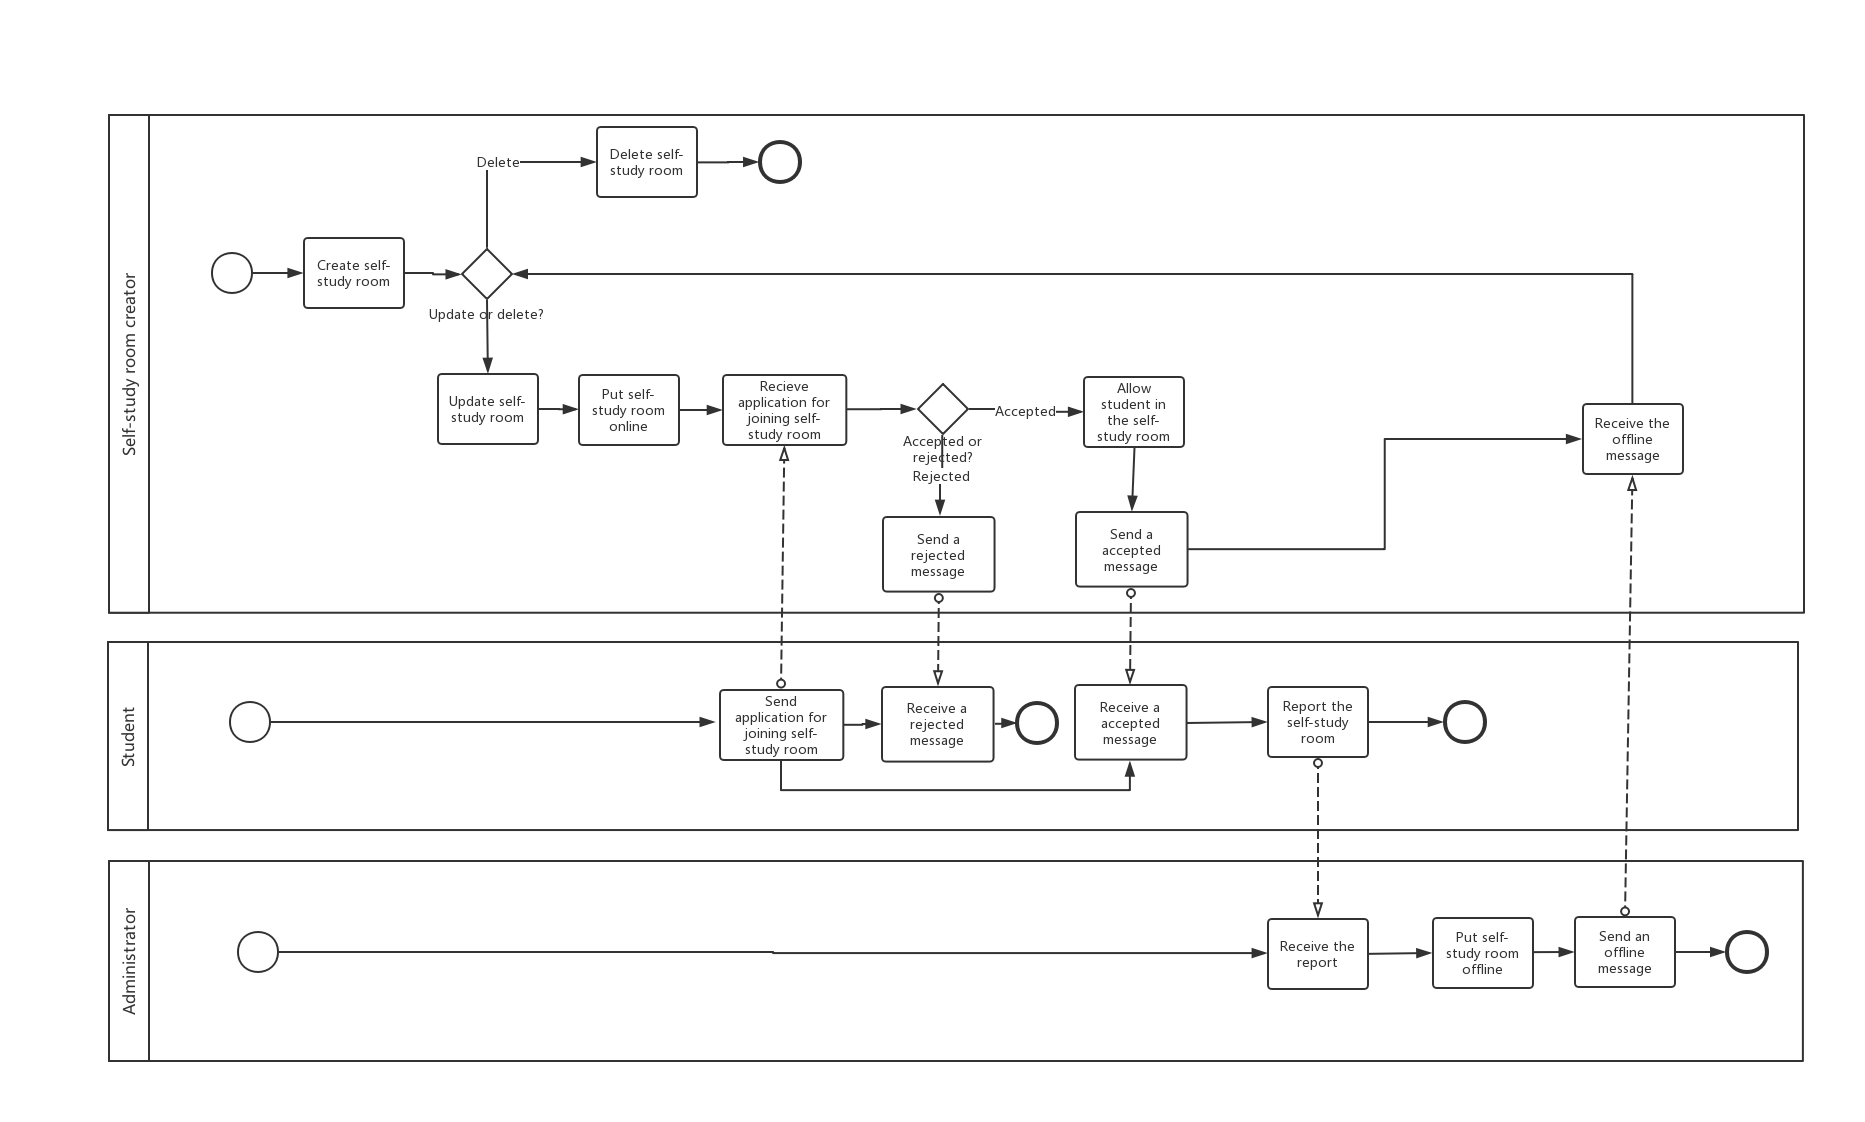
\includegraphics[width=1.0\textwidth]{figure/llt/bpmnselfstudy} %插入图片,[]中设置图片大小,{}中是图片文件名
		\caption{Self Study Service BPMN Model} %最终文档中希望显示的图片标题
		\label{bpmnselfstudy} %用于文内引用的标签
	\end{figure}
	\begin{lstlisting}[language={XML}]
	<cmmn:case id="Case_1">
		<cmmn:casePlanModel id="CasePlanModel_1" name="Report the self-study room">
		<cmmn:planItem id="PlanItem_3" name="Find problems" definitionRef="UserEventListener_1"/>
		<cmmn:planItem id="PlanItem_4" definitionRef="Milestone_1"/>
		<cmmn:stage id="Stage_A" name="Prepare report">
			<cmmn:planItem id="PlanItem_1" definitionRef="HumanTask_A" />
			<cmmn:planItem id="PlanItem_2" definitionRef="HumanTask_B" />
			<cmmn:sentry id="Sentry_1">
				<cmmn:planItemOnPart id="PlanItemOnPart_1" sourceRef="PlanItem_3">
					<cmmn:standardEvent>occur</cmmn:standardEvent>
				</cmmn:planItemOnPart>
			</cmmn:sentry>
			<cmmn:exitCriterion id="ExitCriterion_1" sentryRef="Sentry_2" />
			<cmmn:sentry id="Sentry_2">
				<cmmn:planItemOnPart id="PlanItemOnPart_2" sourceRef="PlanItem_2">
					<cmmn:standardEvent>occur</cmmn:standardEvent>
				</cmmn:planItemOnPart>
			</cmmn:sentry>
			<cmmn:humanTask id="HumanTask_A" name="Take evidence" isBlocking="true">
				<cmmn:planningTable id="PlanningTable_1">
					<cmmn:discretionaryItem id="DiscretionaryItem_1" definitionRef="Check self-study room management rules" />
				</cmmn:planningTable>
			</cmmn:humanTask>
			<cmmn:humanTask id="HumanTask_B" name="Fill in the report" isBlocking="true" />
		</cmmn:stage>
		<cmmn:exitCriterion id="ExitCriterion_2" sentryRef="Sentry_3" />
		<cmmn:milestone id="Milestone_1" name="Report completed" />
		<cmmn:sentry id="Sentry_3">
			<cmmn:planItemOnPart id="PlanItemOnPart_3" sourceRef="Stage_A">
				<cmmn:standardEvent>complete</cmmn:standardEvent>
			</cmmn:planItemOnPart>
		</cmmn:sentry>
	</cmmn:case>

	\end{lstlisting}
	%\clearpage
	%\textbf{Answer Service BPMN Model and XML}\\
	\begin{figure}
		\centering %图片居中
		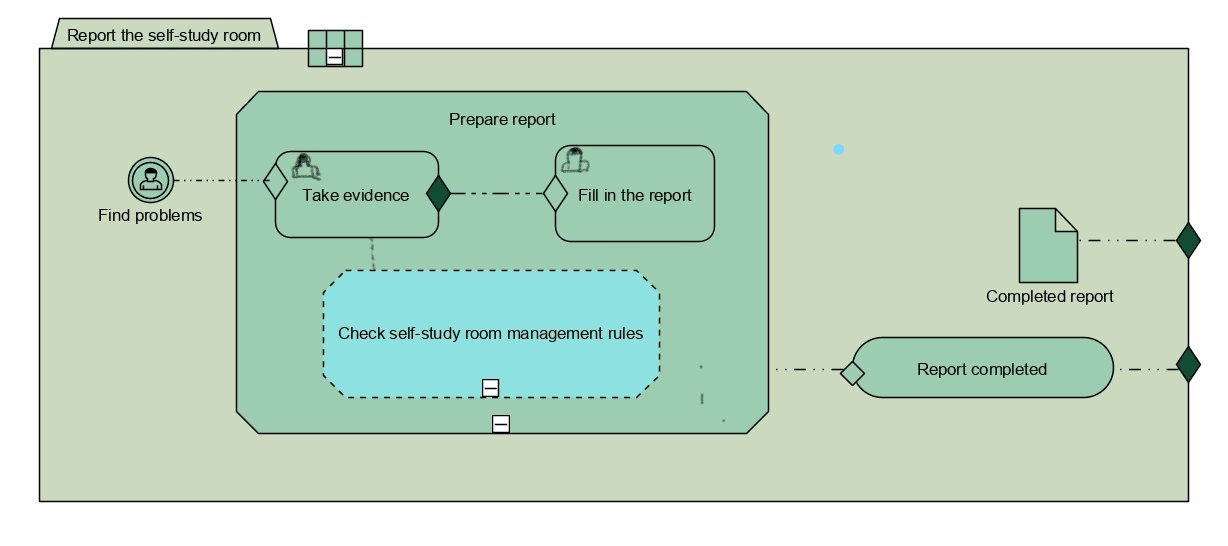
\includegraphics[width=1.0\textwidth]{figure/llt/selfstudyroombpmn} %插入图片,[]中设置图片大小,{}中是图片文件名
		\caption{Studyroom Service BPMN} %最终文档中希望显示的图片标题
		\label{selfstudyroombpmn} %用于文内引用的标签
	\end{figure}
	\begin{lstlisting}[language={XML}]
	<bpmn:process id="Process_2" isExecutable="true">
		<bpmn:startEvent id="StartEvent_1">
	        <bpmn:outgoing>SequenceFlow_1</bpmn:outgoing>
			<bpmn:outgoing>SequenceFlow_5</bpmn:outgoing>
	    </bpmn:startEvent>
		<bpmn:exclusiveGateway id="ExclusiveGateway_1">
			<bpmn:incoming>SequenceFlow_1</bpmn:incoming>
			<bpmn:incoming>SequenceFlow_4</bpmn:incoming>
			<bpmn:outgoing>SequenceFlow_2</bpmn:outgoing>
		</bpmn:exclusiveGateway>
		<bpmn:sequenceFlow id="SequenceFlow_1" sourceRef="StartEvent_1"
	        targetRef="ExclusiveGateway_1" />
		<bpmn:intermediateCatchEvent id="IntermediateCatchEvent_1">
			<bpmn:incoming>SequenceFlow_2</bpmn:incoming>
			<bpmn:outgoing>SequenceFlow_3</bpmn:outgoing>
			<bpmn:timerEventDefinition />
		</bpmn:intermediateCatchEvent>
		<bpmn:sequenceFlow id="SequenceFlow_2" sourceRef="ExclusiveGateway_1"
	        targetRef="IntermediateCatchEvent_1" />
		<bpmn:task id="Task_1" name="Send Reminder">
	        <bpmn:incoming>SequenceFlow_3</bpmn:incoming>
	        <bpmn:outgoing>SequenceFlow_4</bpmn:outgoing>
	    </bpmn:task>
		<bpmn:sequenceFlow id="SequenceFlow_3" sourceRef="IntermediateCatchEvent_1"
	        targetRef="Task_1" />
		<bpmn:sequenceFlow id="SequenceFlow_4" sourceRef="Task_1"
	        targetRef="ExclusiveGateway_1" />
		<bpmn:exclusiveGateway id="ExclusiveGateway_2">
			<bpmn:incoming>SequenceFlow_5</bpmn:incoming>
			<bpmn:outgoing>SequenceFlow_6</bpmn:outgoing>
			<bpmn:outgoing>SequenceFlow_7</bpmn:outgoing>
		</bpmn:exclusiveGateway>
		<bpmn:sequenceFlow id="SequenceFlow_5" sourceRef="StartEvent_1"
	        targetRef="ExclusiveGateway_2" />
		<bpmn:task id="Task_2" name="Send a message to remove the student from the self-study room">
	        <bpmn:incoming>SequenceFlow_6</bpmn:incoming>
	        <bpmn:outgoing>SequenceFlow_8</bpmn:outgoing>
	    </bpmn:task>
		<bpmn:sequenceFlow id="SequenceFlow_6" sourceRef="ExclusiveGateway_2"
			targetRef="Task_2">
			<bpmn:conditionExpression
				xsi:type="bpmn:tFormalExpression">Yes</bpmn:conditionExpression>
		</bpmn:sequenceFlow>
		<bpmn:endEvent id="EndEvent_1">
			<bpmn:incoming>SequenceFlow_8</bpmn:incoming>
		</bpmn:endEvent>
		<bpmn:sequenceFlow id="SequenceFlow_8" sourceRef="Task_2"
	        targetRef="EndEvent_1" />
		<bpmn:task id="Task_3" name="Clock">
	        <bpmn:incoming>SequenceFlow_7</bpmn:incoming>
	        <bpmn:outgoing>SequenceFlow_9</bpmn:outgoing>
	    </bpmn:task>
		<bpmn:sequenceFlow id="SequenceFlow_7" sourceRef="ExclusiveGateway_2"
			targetRef="Task_3">
			<bpmn:conditionExpression
				xsi:type="bpmn:tFormalExpression">No</bpmn:conditionExpression>
		</bpmn:sequenceFlow>
		<bpmn:task id="Task_4" name="Time to learn">
	        <bpmn:incoming>SequenceFlow_9</bpmn:incoming>
			<bpmn:incoming>SequenceFlow_11</bpmn:incoming>
	        <bpmn:outgoing>SequenceFlow_12</bpmn:outgoing>
	    </bpmn:task>
		<bpmn:sequenceFlow id="SequenceFlow_9" sourceRef="Task_3"
	        targetRef="Task_4" />
		<bpmn:boundaryEvent id="BoundaryEvent_1" attachedToRef="Task_4">
			<bpmn:outgoing>SequenceFlow_10</bpmn:outgoing>
			<bpmn:errorEventDefinition />
		</bpmn:boundaryEvent>
		<bpmn:task id="Task_5" name="End this study">
	        <bpmn:incoming>SequenceFlow_10</bpmn:incoming>
	        <bpmn:outgoing>SequenceFlow_11</bpmn:outgoing>
	    </bpmn:task>
		<bpmn:sequenceFlow id="SequenceFlow_10" sourceRef="BoundaryEvent_1"
	        targetRef="Task_5" />
		<bpmn:sequenceFlow id="SequenceFlow_11" sourceRef="Task_5"
	        targetRef="Task_4" />
		<bpmn:intermediateCatchEvent id="IntermediateCatchEvent_2">
			<bpmn:incoming>SequenceFlow_12</bpmn:incoming>
			<bpmn:outgoing>SequenceFlow_13</bpmn:outgoing>
			<bpmn:timerEventDefinition />
		</bpmn:intermediateCatchEvent>
		<bpmn:sequenceFlow id="SequenceFlow_12" sourceRef="Task_4"
	        targetRef="IntermediateCatchEvent_2" />
		<bpmn:task id="Task_6" name="Display statistics report">
	        <bpmn:incoming>SequenceFlow_13</bpmn:incoming>
	        <bpmn:outgoing>SequenceFlow_14</bpmn:outgoing>
	    </bpmn:task>
		<bpmn:sequenceFlow id="SequenceFlow_13" sourceRef="IntermediateCatchEvent_2"
	        targetRef="Task_6" />
		<bpmn:endEvent id="EndEvent_2">
			<bpmn:incoming>SequenceFlow_14</bpmn:incoming>
		</bpmn:endEvent>
		<bpmn:sequenceFlow id="SequenceFlow_14" sourceRef="Task_6"
	        targetRef="EndEvent_2" />
	</bpmn:process>
	
	\end{lstlisting}
	\clearpage
	\begin{figure}
		\centering %图片居中
		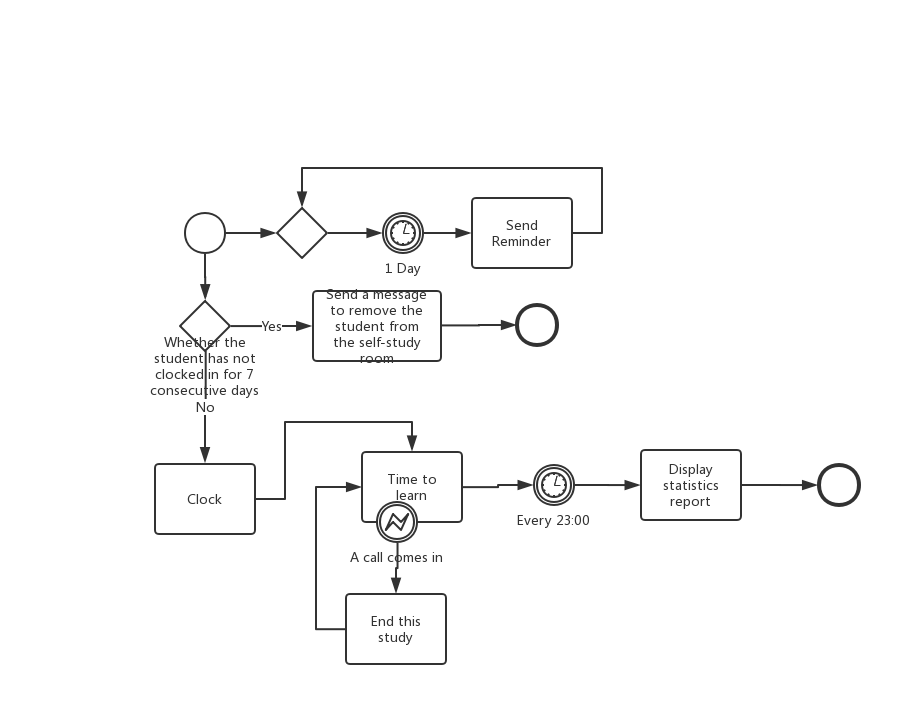
\includegraphics[width=1.0\textwidth]{figure/llt/attendanceservicebpmn} %插入图片,[]中设置图片大小,{}中是图片文件名
		\caption{Attendance Service BPMN} %最终文档中希望显示的图片标题
		\label{attendanceservicebpmn} %用于文内引用的标签
	\end{figure}

	\begin{figure}
		\centering %图片居中
		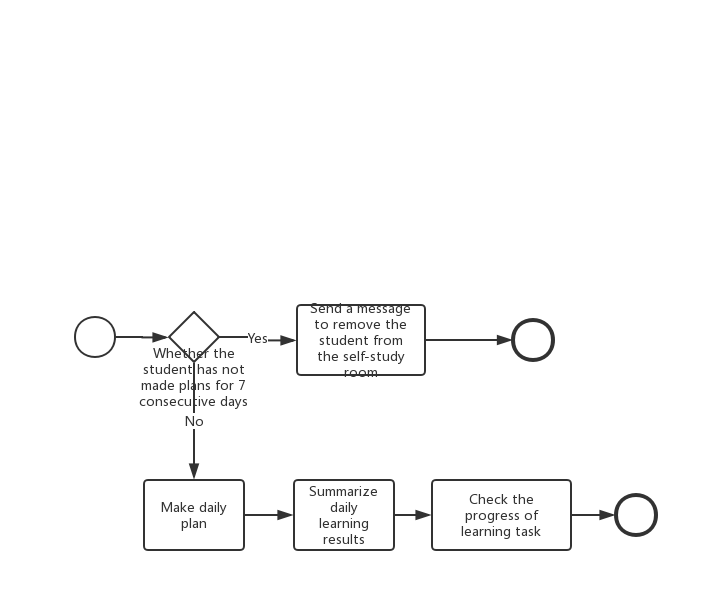
\includegraphics[width=1.0\textwidth]{figure/llt/learningtaskservice} %插入图片,[]中设置图片大小,{}中是图片文件名
		\caption{Learning Task Service} %最终文档中希望显示的图片标题
		\label{learningtaskservice} %用于文内引用的标签
	\end{figure}
	\begin{lstlisting}[language={XML}]
	<bpmn:process id="Process_3" isExecutable="true">
		<bpmn:startEvent id="StartEvent_1">
	        <bpmn:outgoing>SequenceFlow_1</bpmn:outgoing>
	    </bpmn:startEvent>
		<bpmn:exclusiveGateway id="ExclusiveGateway_1">
			<bpmn:incoming>SequenceFlow_1</bpmn:incoming>
			<bpmn:outgoing>SequenceFlow_4</bpmn:outgoing>
			<bpmn:outgoing>SequenceFlow_2</bpmn:outgoing>
		</bpmn:exclusiveGateway>
		<bpmn:sequenceFlow id="SequenceFlow_1" sourceRef="StartEvent_1"
	        targetRef="ExclusiveGateway_1" />
		<bpmn:task id="Task_1" name="Send a message to remove the student from the self-study room">
	        <bpmn:incoming>SequenceFlow_2</bpmn:incoming>
	        <bpmn:outgoing>SequenceFlow_3</bpmn:outgoing>
	    </bpmn:task>
		<bpmn:sequenceFlow id="SequenceFlow_2" sourceRef="ExclusiveGateway_1"
			targetRef="Task_1">
			<bpmn:conditionExpression
				xsi:type="bpmn:tFormalExpression">Yes</bpmn:conditionExpression>
		</bpmn:sequenceFlow>
		<bpmn:endEvent id="EndEvent_1">
			<bpmn:incoming>SequenceFlow_3</bpmn:incoming>
		</bpmn:endEvent>
		<bpmn:sequenceFlow id="SequenceFlow_3" sourceRef="Task_1"
	        targetRef="EndEvent_1" />
		<bpmn:task id="Task_2" name="Make daily plan">
	        <bpmn:incoming>SequenceFlow_4</bpmn:incoming>
	        <bpmn:outgoing>SequenceFlow_5</bpmn:outgoing>
	    </bpmn:task>	
		<bpmn:sequenceFlow id="SequenceFlow_4" sourceRef="ExclusiveGateway_1"
	        targetRef="Task_2" />
		<bpmn:task id="Task_3" name="Summarize daily learning results">
	        <bpmn:incoming>SequenceFlow_5</bpmn:incoming>
	        <bpmn:outgoing>SequenceFlow_6</bpmn:outgoing>
	    </bpmn:task>	
		<bpmn:sequenceFlow id="SequenceFlow_5" sourceRef="Task_2"
	        targetRef="Task_3" />
		<bpmn:task id="Task_4" name="Check the progress of learning task">
	        <bpmn:incoming>SequenceFlow_6</bpmn:incoming>
	        <bpmn:outgoing>SequenceFlow_7</bpmn:outgoing>
	    </bpmn:task>	
		<bpmn:sequenceFlow id="SequenceFlow_6" sourceRef="Task_3"
	        targetRef="Task_4" />
		<bpmn:endEvent id="EndEvent_2">
			<bpmn:incoming>SequenceFlow_7</bpmn:incoming>
		</bpmn:endEvent>
		<bpmn:sequenceFlow id="SequenceFlow_7" sourceRef="Task_4"
	        targetRef="EndEvent_2" />
	</bpmn:process>

	\end{lstlisting}
	
	\clearpage

\end{document}
